\documentclass[nosignatures]{mscThesis}


\usepackage[table]{xcolor}
\RequirePackage{siunitx}
\RequirePackage[T1]{fontenc}                        % T1 font encoding for PDFs
\RequirePackage{lmodern}                                % extended font definition
\RequirePackage{amsmath,amssymb,amsthm} % most important math stuff
\RequirePackage{a4wide}                                 % make better use of A4 paper
\RequirePackage{fancyhdr}                               % custom headers and footers
\RequirePackage{fncychap}                               % custom chapter titles
\RequirePackage{graphicx}                               % graphics
\RequirePackage{color}                                  % color
\RequirePackage{booktabs}                               % extra tabular commands
\RequirePackage[format=plain]{caption}  % improved caption format
\RequirePackage{nomencl}                                % cool nomenclature listing
\RequirePackage{makeidx}                                % create your index
\RequirePackage[printonlyused]{acronym}
\RequirePackage{ifthen}                                 % if-then commands (used in maketitle)
\RequirePackage{eso-pic}                                % picture in back/forground (used in cover)
\RequirePackage{relsize}                                % \textlarger, \textsmaller etc
%%
%%
%%%%%%%%%%%%%%%%%%%%%%%%%%%%%%%%%%%%%%%%%%%%%%%%%%%%%%%%%%%%
%%
%%  Set up Matlab and C++ Listings
%%  REQUIRES PACKAGE listings AND colortbl
%%
%%%%%%%%%%%%%%%%%%%%%%%%%%%%%%%%%%%%%%%%%%%%%%%%%%%%%%%%%%%%
%%
%%
\RequirePackage{listings}%

\usepackage[utf8]{inputenc}

\usepackage{pgf,tikz}

\usepackage{pgfgantt}

\usepackage{mathrsfs}

\usepackage{mathtools}

\usepackage{gensymb}

\usepackage{float}

\usepackage{needspace}

\usepackage{pgfplots}

\usepackage[nodayofweek,level]{datetime}

\usepackage{todonotes}

\usepackage{bm}

\usepackage{enumitem}

\usepackage{graphicx}

\usepackage{subcaption}

\usepackage{indentfirst}

\usepackage{multirow}

\usepackage{eurosym}

\usepackage{hhline}

\usepackage[nameinlink,noabbrev]{cleveref}

\usepackage{upgreek}

\usetikzlibrary{arrows}

\setlength{\parindent}{15pt}

\pgfplotsset{compat=newest}
%prevent sections from starting if there is not enough space
\let\oldsection\section
\renewcommand\section{\Needspace{10\baselineskip}\oldsection}
\let\oldsubsection\subsection
\renewcommand\subsection{\Needspace{10\baselineskip}\oldsubsection}

\DeclareMathOperator*{\argmin}{argmin}   % Jan Hlavacek

\creflabelformat{equation}{#2#1#3}

\newtagform{noparen}{}{}
\usetagform{noparen}


\DeclareSIUnit{\EURO}{\text\euro}
\captionsetup{justification=centering}

%\hypersetup{colorlinks=false}
\newcommand{\code}[1]{\texttt{#1}}



%this makes it possible to include latex inside SI
\sisetup{parse-numbers = false, number-math-rm = \ensuremath, per-mode=symbol}
\usetikzlibrary{quotes,arrows.meta}
\tikzset{
	annotated cuboid/.pic={
		\tikzset{%
			every edge quotes/.append style={midway, auto},
			/cuboid/.cd,
			#1
		}
		\draw [every edge/.append style={pic actions, densely dashed, opacity=.5}, pic actions]
		(0,0,0) coordinate (o) -- ++(-\cubescale*\cubex,0,0) coordinate (a) -- ++(0,-\cubescale*\cubey,0) coordinate (b) edge coordinate [pos=1] (g) ++(0,0,-\cubescale*\cubez)  -- ++(\cubescale*\cubex,0,0) coordinate (c) -- cycle
		(o) -- ++(0,0,-\cubescale*\cubez) coordinate (d) -- ++(0,-\cubescale*\cubey,0) coordinate (e) edge (g) -- (c) -- cycle
		(o) -- (a) -- ++(0,0,-\cubescale*\cubez) coordinate (f) edge (g) -- (d) -- cycle;
		\path [every edge/.append style={pic actions, |-|}]
		(b) +(0,-5pt) coordinate (b1) edge ["$\vec{dim}(1)$"'] (b1 -| c)
		(b) +(-5pt,0) coordinate (b2) edge ["$\vec{dim}(3)$"] (b2 |- a)
		(c) +(3.5pt,-3.5pt) coordinate (c2) edge ["$\vec{dim}(2)$"'] ([xshift=3.5pt,yshift=-3.5pt]e)
		; \path (b)++(\cubescale*\cubex/2,0,0)++(0,0,-\cubescale*\cubez/2) coordinate(x);
		\draw[->] (x)--++(\cubescale*\cubex/5,0,0) node[anchor=west]{$x$};
		\draw[->] (x)--++(0,\cubescale*\cubex/5,0) node[anchor=south]{$z$};
		\draw[->] (x)--++(0,0,-\cubescale*\cubex/5) node[anchor=west]{$y$};
	},
	/cuboid/.search also={/tikz},
	/cuboid/.cd,
	width/.store in=\cubex,
	height/.store in=\cubey,
	depth/.store in=\cubez,
	units/.store in=\cubeunits,
	scale/.store in=\cubescale,
	width=10,
	height=10,
	depth=10,
	units=cm,
	scale=.1,
}

%redefine vector and Real symbols for faster typing
\renewcommand{\vec}[1]{\bm{#1}}
\newcommand{\R}{\mathbb R}
\newcommand{\Z}{\mathbb Z}
\newcommand{\foralli}[1][]{\forall i \in \{1\dots n_{#1}\}}
\newcommand{\forallj}[1][]{\forall j \in \{1\dots n_{#1}\}}
\newcommand{\forallk}[1][]{\forall k \in \{1\dots n_{#1}\}}
\newcommand{\dott}[1]{\frac{\partial #1}{\partial t}}
\newcommand{\ddott}[1]{\frac{\partial ^2 #1}{\partial t^2}}
\newcommand{\torque}{\Upgamma}

\newcommand{\mat}[2][b]{\begin{#1matrix}#2\end{#1matrix}}

%set spacing between rows in tables
\renewcommand{\arraystretch}{1.2}


\mscDepartment{Delft Center for Systems and Control (\textsmaller{DCSC})}%
\mscProgram{Systems and Control}
%Change if needed to
%\mscProgram{Mechanical Engineering}
\mscFaculty{Mechanical, Maritime and Materials Engineering (3mE)}%
%
%-name, date, title
\mscName{Iñigo Moreno Caireta}%
\mscDate{\today}%
\mscTitle{Planng and Control of a Multiple-Quadcopter System Cooperatively Carrying a Slung Payload in Dynamical Environments}%
\mscSubTitle{A Centralized Model Predictive Control Solution}%
\mscKeyWords{thesis, msc, subject}% only used in PDF properties
%
%-cover picture
\mscCoverPicture{STYLESTUFF/COVER}% to place a picture ( here the example COVER.eps) on the cover page. Comment out if no picture is to be used
%
%
%-Third party options (create text/logo on the copywrite page)
\mscThirdPartyText{}
\mscThirdPartyLogo{}
%
%	
% The examination committee  - Supervisors and Readers
\mscSupervisorOne{Lluis Ros}
\mscSupervisorTwo{Mercè Ollé}
%\mscSupervisorThree{}
%\mscReaderFour{}
%
% Finalize the thesis data
\setThesisInfo
%
% Use \includeonly{} to build only certain parts of your thesis
%\includeonly{introduction, real_chapter, empty_chapter, long_chapter}%
%
% allow (matlab, C++ etc) listing max 1pt flexibility between lines
\lstset{lineskip=0pt plus 1pt minus 0pt} %%
%
\begin{document}
%
%========================== Front matter ======================================
\frontmatter %
%
% Make the cover page and hell of a lot of title pages
\maketitle
%
%
% Abstract (does not appear in the Table of Contents)
\chapter*{Abstract}%

%\acp{UAV} have been thoroughly used for transportation in unpredictable environments. However, one of the limits for these applications is usually the payload mass, as it cannot be too big in relation to the drones' mass. In this thesis, we propose the use of multiple drones for cooperative transportation through strings. In contrast with current approaches for the control of such systems, we propose the use of \ac{NMPC} to achieve more aggressive and agile maneuvers. The control algorithm's effectiveness is demonstrated in simulated environments. 

Lorem ipsum dolor sit amet, consectetur adipiscing elit, sed do eiusmod tempor incididunt ut labore et dolore magna aliqua. Ut enim ad minim veniam, quis nostrud exercitation ullamco laboris nisi ut aliquip ex ea commodo consequat. Duis aute irure dolor in reprehenderit in voluptate velit esse cillum dolore eu fugiat nulla pariatur. Excepteur sint occaecat cupidatat non proident, sunt in culpa qui officia deserunt mollit anim id est laborum.






% table of contents, (\toc of \toclof of \tocloflot )
\setcounter{tocdepth}{2}
%\tocloflot
\toclof
%
%
%%
% Preface

\chapter{Preface}

\todo{Write or remove preface}

Lorem ipsum dolor sit amet, consectetur adipiscing elit. Quisque vitae fermentum quam. Sed a velit vel lectus convallis semper sed quis turpis. In hac habitasse platea dictumst. Maecenas velit nunc, sagittis eu tortor at, porta interdum eros. Nullam commodo metus eros, nec porta risus tempor eget. Nullam lobortis, eros eget vestibulum porttitor, mauris velit aliquet arcu, in semper erat leo ac eros. Cras eget felis pulvinar, iaculis justo quis, volutpat turpis. Donec fringilla diam nec nisi tincidunt, dictum imperdiet sapien pellentesque.




%%
% Acknowledgements
\chapter{Acknowledgements}%
\todo{write or remove acknowledgements}
Lorem ipsum dolor sit amet, consectetur adipiscing elit. Quisque vitae fermentum quam. Sed a velit vel lectus convallis semper sed quis turpis. In hac habitasse platea dictumst. Maecenas velit nunc, sagittis eu tortor at, porta interdum eros. Nullam commodo metus eros, nec porta risus tempor eget. Nullam lobortis, eros eget vestibulum porttitor, mauris velit aliquet arcu, in semper erat leo ac eros. Cras eget felis pulvinar, iaculis justo quis, volutpat turpis. Donec fringilla diam nec nisi tincidunt, dictum imperdiet sapien pellentesque.



\vspace*{15mm}

Delft, University of Technology \hfill \mscname \\
\mscdate
%%
% Dedication page. 
\cleardoublepage
\thispagestyle{empty}
\vspace*{\stretch{1}}

% Put your own motto here, or dedicate your work to your Mom or whatever...
\begin{quote}
\noindent``Lorem ipsum dolor sit amet, consectetur adipiscing elit. Quisque vitae fermentum quam. Sed a velit vel lectus convallis semper sed quis turpis.

''
	
--- \emph{Lorem Ipsum}
\end{quote}
\todo{Choose or remove quote}

\vspace{\stretch{3}}
\clearemptydoublepage
%
%========================== Main matter ======================================
\mainmatter
%
%
% Introduction
\chapter{Introduction} \label{chap::intro}

\section{Theme Relevance and Justification}

\subsection{Omni-wheeled robots}

\subsection{Model Predictive Control}

\section{Research Objective}
The objective of the research included in this thesis is to:

\begin{quote}
	\emph{
		Design a control algorithm for systems with an omni-wheeled robot and demonstrate it in simulated and real scenarios.
	}
\end{quote}

\section{Thesis Context}

This thesis is a result of the collaboration between \ac{FME} and \ac{IRI}. During the summer of 2018 I contacted \mscsupervisorone looking for a suitable project for my Master's Thesis and he proposed me this one.

\section{Notation}

Throughout this thesis the following notation will be used:

\setlength\arrayrulewidth{1.2pt}
\let\oldarraystretch\arraystretch
\renewcommand{\arraystretch}{1.2}
%\rowcolors{2}{gray!10}{white}
\begin{table}[H]
\begin{center}
\begin{tabular}{ l | c | c }
	& Symbol & Definition \\\hline
	Scalars: & $x$ & \\ 
	Vectors: & $\vec{x}$ & \\  
	Elements of vector: & $\vec{x}(i)$ & $i$-th element of vector $\vec x$\\ 
	Position vectors: & $\vec p_x$ & \\
	Coordinates of position vector: &$x_x, y_x, z_x$&x,y,z coordinates of position $\vec p_x$\\
	Matrices: & $\vec{X}$ & \\
	Sets: & $\mathcal{X}$ & \\
	%Set of unit vectors: & $\mathcal{S}^{n-1}$ & $\{\vec{x}\in \R^n | \ \|\vec{x}\|=1\}$ \\
	Time derivatives: & $\dot{x}$ & $\frac{\partial x}{\partial t}$ \\
	Desired values: & $\bar{x} $&  desired value of $x$ \\
	Predicted values: & $\hat{x} $&  predicted value of $x$ 
	%Set of positive semidefinite matrices of size $n$: & $\mathcal{S}^n_+$ & $\{\vec{A\in\R^{n\times n}}| \ \vec{x}^T\vec{Ax}>0 \ \forall \ x\in \R_{\ne 0}^n\}$\\ 
	%Weighted squared norm: & $\|\vec{x}\|_{\vec{Q}}$ & $\vec{x}^T\vec{Qx} \ \forall \  \vec{x}\in\R^n ,\ \vec{Q}\in \mathcal{S}^n_+ $ \\
%	Hat map: & $\hat{x}$ & $\hat{x} y=x\times y \ \forall \ x,y\in\R^3$
	\label{tab:Notation}
\end{tabular}
\caption{Thesis Notation}
\end{center}
\end{table}
All vectors are column vectors and all positions are expressed in the \ac{ENU} inertial frame unless otherwise stated.




\let\arraystretch\oldarraystretch



%
% Problem
\chapter{Problem Formulation} \label{chap::problem}


\section{Omni-wheeled robot} \label{sect::system}
The robot can be represented as a rigid body in a planar space. The location of the robot's \ac{COM} is defined as \lsymb{$\vec p_0\in\R^2$}{Location of the robot's center point} and the yaw of the robot is represeted as \gsymb{$\psi\in\R$}{Roll of the robot}.

Assuming the robot has \lsymb{$n\in\Z_{> 0}$}{Number of wheels} wheels, we can define their 


\section{Dynamic Model}

\newpage
\subsection{Motor Dynamics Identification}

The motors in our robot are controlled by velocity inputs. We will represent the inputs of the i-th motor as \lsymb{$u_i\in[-1,1]$}{i-th motor input}. The motors are also equipped with encoders from which we can deduce the angle of each wheel, denoted as \gsymb{$theta_i\in\R$}{i-th wheel angle}.

We can try to identify the model using process model identification. A tool that, given some identification data and a transfer function with unknown parameters, estimates the value of the parameters. We will assume that the relationship between input velocity and the real velocity follow a linear transfer function:
\begin{equation}
\frac{\dot{\theta_i}(s)}{u_i(s)}=\frac{K_i}{1+\tau_i s}
\rightarrow
\frac{\theta_i(s)}{u_i(s)}=\frac{K_i}{s(1+\tau_i s)}
\end{equation}

Which corresponds to the following set of ODEs:
\begin{equation}
\dot{\theta_i}+\tau\ddot{\theta_i}=u\,K
\end{equation}

To obtain the identification data we can make the arduino generate a square wave and record the data from the encoder. This will give us data discretized with different time-intervals as the time-interval will depend on the loop size. To get data with equal time-intervals we can set a higher sampling frequency and interpolate the values between each sample.

When identifying the model we saw that the values of $K$ were different for varying amplitudes as we can see in \cref{fig:K_u}.

\todo{Do experiments for higher values of amplitude (when lab is empty)}
\begin{figure}[h]
	\centering
	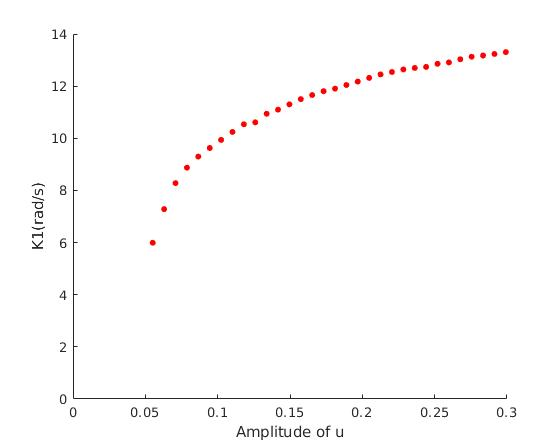
\includegraphics[width=0.31415\textwidth]{Figures/K_u}
	\caption{Relationship between $K_1$ and the amplitude of $u$}
	\label{fig:K_u}
\end{figure}


As the relationship looks like it has a vertical and a horizontal asymptote, we will try to model it with a rational function of the form:
\begin{equation}
K_i=\frac{a_i\,u_i+b_i}{u_i+c_i}
\end{equation}

\begin{figure}[h]
	\centering
	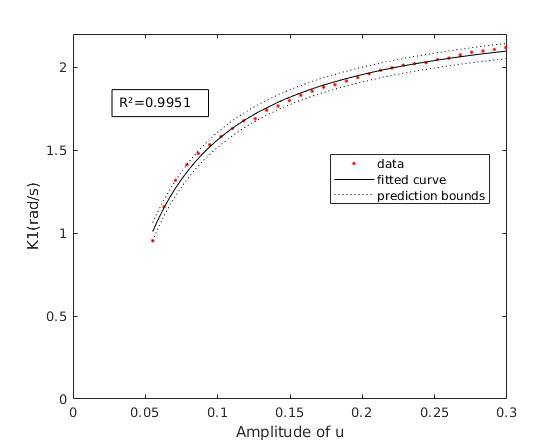
\includegraphics[width=0.31415\textwidth]{Figures/K_u_pred}
	\caption{Predicted relationship between $K_1$ and the amplitude of $u$}
	\label{fig:K_u_pred}
\end{figure}
\todo{see if $\tau$ depends on u}






\subsection{Aerodynamic Drag}
We will use the same model for aerodynamic drag model as in \cite{Potdar2018}. The drag on the payload, denoted as \lsymb{$\vec F_{Dl}\in\R^3$}{Aerodynamic drag on the payload}, is modeled using a quadratic drag model, while the drag on each quadrotor, denoted as \lsymb{$\vec F_{Di}\in\R^3$}{Aerodynamic drag on the $i$-th drone}, is modeled using a linear drag model.
\begin{alignat}{2}
\vec F_{Dl} &= 
-k_{Dl}\|\dot{\vec p}_l\|^2\frac{\dot{\vec p}_l}{\|\dot{\vec p}_l\|} &&= 
-k_{Dl}\|\dot{\vec p}_l\|\dot{\vec p}_l
\label{eq::dragl}
\\
\vec F_{Di} &= 
-k_{Di}\|\dot{\vec p}_i\|\frac{\dot{\vec p}_i}{\|\dot{\vec p}_i\|} &&= 
-k_{Di}\dot{\vec p}_i \quad\foralli
\label{eq::dragi}
\end{alignat}

Where \lsymb{$k_{Dl}\in\R$}{Drag constant of the payload} and \lsymb{$k_{Di}\in\R$}{Drag constant of the $i$-th quadrotor} are the drag constants identified in \cite{Potdar2018}.

\subsubsection{Drag Inclusion in \ac{EOMs}}
To use include drag in our problem we need to include the drag force calculated in equations \ref{eq::dragl} and \ref{eq::dragi} in the \ac{EOMs} declared in equations \ref{eq::eom2} and \ref{eq::eom3}.

The drag force on the drones $\vec F_{Di}$ can be added to the input force $\vec F_{ui}$ (we will denote this sum as \lsymb{$\vec F_{uDi}$}{addition of $\vec F_{ui}$ and $\vec F_{Di}$}). The drag force on the payload can be included by subtracting $\frac{\vec F_{Dl}}{m_l}$ from all appearances of $\ddot{\vec p}_l$ in the \ac{EOMs}, in the same way that $g\vec e_3$ is subtracted. The resulting \ac{EOMs} from these changes are:


\begin{align}
\dot{\vec q}_i& = \vec w_i \times \vec q_i \quad \foralli \label{eq::eom_drag1}
\\
\vec M_q(\ddot{\vec p}_l-g \vec e_3-\frac{\vec F_{Dl}}{m_l}) &= \sum_{i=1}^{n}(-m_il_i\|\vec w_i\|^2\vec q_i +\vec F_{uDi}^\parallel) \label{eq::eom_drag2}
\\
\dot{\vec w}_i &=\frac{1}{l_i}\vec q_i\times(\ddot{\vec p}_l-g \vec e_3-\frac{\vec F_{Dl}}{m_l})-\frac{1}{m_il_i}(\vec q_i\times\vec F_{uDi}^\perp) \quad \foralli \label{eq::eom_drag3}
\end{align}

\subsection{Environment Definition}
The environment is defined as a 3 dimensional box with the origin in the floor's center. We denote the box's dimensions as \lsymb{$\vec{dim}\in\R^3_{>0}$}{Environment dimensions}. A schematic of the environment can be seen in \cref{fig::environment}.

\begin{figure}
	\centering
	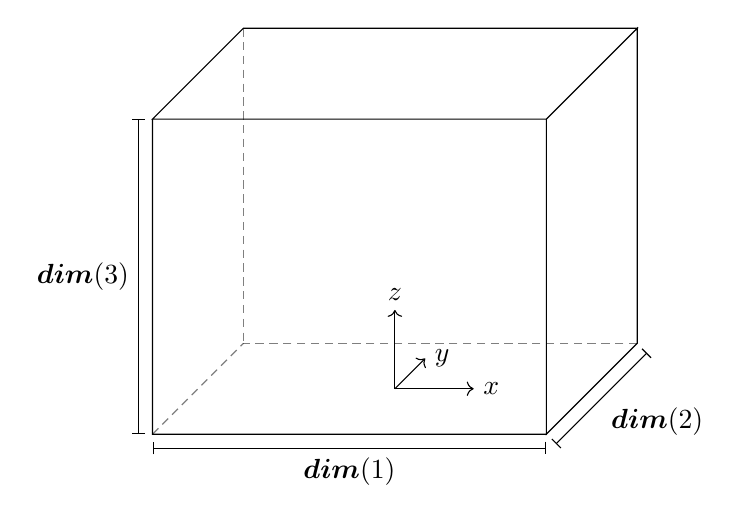
\begin{tikzpicture}
	\pic at (1,-3) {annotated cuboid={width=250, height=200, depth=150, scale=.02, units=m}};
	\end{tikzpicture}
	\caption{Environment Schematic}
	\label{fig::environment}
\end{figure}


\subsection{Obstacle Modeling}
\label{subsect::obstacle_modeling}
Obstacles are modeled as three dimensional boxes and their behavior is modeled as linear movement using a Kalman Filter. This is required so that the planner takes into account future movement of the obstacles. The number of obstacles is denoted by \lsymb{$n_{obs}\in\Z_{\ge0}$}{Number of obstacles}, their center position by \lsymb{$\vec{p}_{obs_i}\in\R^3$}{Position of the $i$-th obstacle} and their dimension by \lsymb{$\vec{dim}_{obs_i}\in\R^3_{>0}$}{Dimension of the $i$-th obstacle}. 

Often we will use the smallest ellipsoid that contains the box.  The equations to find the radial dimensions of the ellipsoid (denoted as \lsymb{$\vec{dim}_{ell_i}\in\R^3$}{Ellipsoid dimensions of the $i$-th obstacle}) are:

\begin{figure}
\usetikzlibrary{decorations.pathreplacing}
\centering
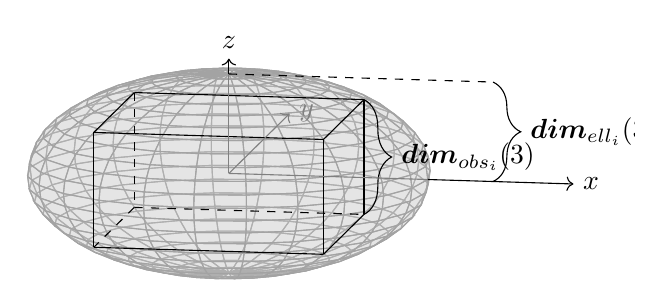
\begin{tikzpicture}
\begin{axis}[%
width=0.8\textwidth,
axis equal,
view={10}{10},
axis lines = none,
xmax=3,
ymax=3,
zmax=1,
ticks=none,
colormap={}{ gray(0cm)=(0.8); gray(1cm)=(0.8);}
]
\addplot3[%
fill opacity=0.3,
surf,
domain=0:2*pi,y domain=0:pi,
z buffer=sort
]
({sqrt(3)*1*cos(deg(x))*sin(deg(y))}, {sqrt(3)*1 *sin(deg(x))*sin(deg(y))}, {sqrt(3)*.5*cos(deg(y))});
\draw (-1,1,.5)--(1,1,.5);
\draw (-1,-1,.5)--(1,-1,.5);
\draw[dashed] (-1,1,-.5)--(1,1,-.5);
\draw (-1,-1,-.5)--(1,-1,-.5);

\draw (1,1,.5)--(1,-1,.5);
\draw (-1,1,.5)--(-1,-1,.5);
\draw (1,1,-.5)--(1,-1,-.5);
\draw[dashed] (-1,1,-.5)--(-1,-1,-.5);

\draw (1,1,.5)--(1,1,-.5);
\draw[dashed] (-1,1,.5)--(-1,1,-.5);
\draw (1,-1,.5)--(1,-1,-.5);
\draw (-1,-1,.5)--(-1,-1,-.5);

\draw[decorate,decoration={brace,amplitude=10pt,mirror}] (1,1,-.5)--(1,1,.5) node[midway,anchor=west,xshift=10pt]{$\vec{dim}_{obs_i}(3)$};
%\node[anchor=west] at (1.1,1,0) {$\vec{dim}_{obs_i}(3)$};
\draw[dashed] (0,0,.866)--(2.3,0,.866);
\draw[decorate,decoration={brace,amplitude=10pt}] (2.3,0,.866)--(2.3,0,0) node[midway,anchor=west,xshift=10pt]{$\vec{dim}_{ell_i}(3)$};


\draw[color=gray] (0,0,0)--(1.732,0,0);
\draw[->] (1.732,0,0)--(3,0,0) node[anchor=west]{$x$};

\draw[->,color=gray] (0,0,0)--(0,3,0) node[anchor=west]{$y$};


\draw[color=gray] (0,0,0)--(0,0,.866);
\draw[->] (0,0,.866)--(0,0,1) node[anchor=south]{$z$};
\end{axis}
%
\end{tikzpicture}
\caption{Obstacle dimensions}
\label{fig::obstacle_dimensions}

\end{figure}

\begin{equation}
\vec{dim}_{ell_i} = \frac{\sqrt{3}}{2}\vec{dim}_{obs_i}
\quad\foralli[obs]
\end{equation}

A schematic of an obstacle and its dimensions can be seen in \cref{fig::obstacle_dimensions}. For further explanation refer to his thesis\cite{Potdar2018}.
%\chapter{\ac{MPC} Formulation}

An \ac{MPC} problem consists of a state vector which can be modified by a certain input following a set of inter-state equalities. The \ac{MPC} repeats these equalities, generating a fixed number (\lsymb{$N\in\Z_+$}{Number of stages hin the \ac{MPC} formulation}) of predicted stages. An objective function is defined which evaluates the performance of these stages. The \ac{MPC} solver finds, iteratively, the inputs that minimize this objective function. The search space can also be limited using constraints on the state vector.

In our case, the inter-state equalities are the discretization of the dynamics defined previously with a fixed time-delta (denoted as \lsymb{$\Delta t\in\R_+$}{Time between stages in the \ac{MPC} formulation}). This discretization is done using the \ac{RK2} method. Therefore, each stage represents a time in the future and they are separated by $\Delta t$.

The number of iterations that the solver will try to find the optimal solution depends on how difficult the problem is in each stage and is highly variable. However, we can limit it by a maximum number of iterations (denoted as \lsymb{$n_{maxit}\in\Z_+$}{Maximum number of iterations of the \ac{MPC} solver}).

\section{Formal Definition}
The formal definition of the \ac{MPC} problem is:
\begin{align}
\begin{array}{c l r}
\underset{u_1,u_2\dots u_N}{\argmin} & \sum_{k=1}^{N}C(\vec x_k,\vec u_k,\vec s_k) & \text{(Cost Function)}\\\arrayrulecolor{lightgray}\hline
\text{s.t.} & \vec x_1 = \vec x(t) & \text{(Inital condition)}\\
& \vec x_{k+1} = f(\vec x_k,\vec u_k) & \text{(Discretised dynamics)}\\
&I(\vec x_k,\vec u_k,\vec s_k) \ge \vec 0 &  \text{(Constraints)}
\end{array}
\label{eq::formal_def}
\end{align}

\section{Election of State Variables}
To be able to use these dynamics in the \ac{MPC} problem, we need to create a state vector and write code to generate its derivative given the state and inputs.

It is important to choose the state vector correctly so that the number of variables is minimized and singularities are prevented. 

Throughout this thesis, we will denote the number of variables as \lsymb{$n_{var}\in\Z_{> 0}$}{Number of variables in the state vector} and the state vector as \others{$\vec{x}\in\R^{n_{var}}$}{State vector}.

Considering the system definition introduced in section \ref{sect::system}, the most straightforward approach to choosing the state vector is the following:
\begin{equation}
\vec{x}=
[\vec p_l ,\quad
 \vec q_1 \dots \vec q_i \dots \vec q_n ,\quad
 \vec{\dot{p}}_l ,\quad
 \vec w_1 \dots \vec w_i \dots \vec w_n ,\quad
 \vec{ss}_1 \dots \vec{ss}_i \dots \vec{ss}_n
]
\label{eq::state_naive}
\end{equation}

\subsection{Reducing $q_i$}
However, as introduced in \cite{Potdar2018} it is best to use payload angles for the state vector, as they reduce the number of variables. These angles are represented in \cref{fig::angles} and are denoted by \gsymb{$\vartheta_i\in\R$}{First payload angle of the $i$-th quadrotor} and \gsymb{$\varphi_i\in\R$}{Second payload angle of the $i$-th quadrotor}. Using these angles we can define each of the $\vec q_i$ vectors in the following way:

\usetikzlibrary{calc} 
\begin{figure}
\centering
\begin{tikzpicture}[rotate around x=-90]
\draw[->] (0,0,0) -- (1,0,0) node[anchor=west]{x};
\draw[->] (0,0,0) -- (0,1,0) node[anchor=west]{y};
\draw[->] (0,0,0) -- (0,0,1) node[anchor=south]{z};
\coordinate (q) at (.4,.4,3);
\draw (q)+(-5.5pt,-3pt) node{
\includegraphics{Figures/quad}};

\def\a{1.5}
\def\p{3}
\draw[->,thick] (q) -- +(\a,\a,-\p) coordinate(l) node[midway,anchor=south west]{$\vec q_i$};

\draw[densely dotted] (q) -- +(0,0,-\p) (q) -- +(\a,0,-\p) (q) -- ++(\a,\a,-\p) coordinate(c) -- ++(0,-\a,0) coordinate(b) -- ++(-\a,0,0) coordinate(a);

\draw[loosely dotted] (q) -- ++(0,\a ,-\p) -- +(0,-\a,0) +(0,0,0) --  +(\a,0,0);

\draw[->] ($(q)!50pt!(a)$) coordinate(pha) to[out=0,in=206.5] ($(q)!50pt!(b)$) coordinate(phb);

\draw[->] ($(q)!70pt!(b)$) coordinate(tha) to[out=26.5,in=220] ($(q)!70pt!(c)$) coordinate(thb);

\draw ($(phb)!.5!(pha)$) node[anchor=north]{$\varphi_i$};
\draw ($(thb)!.5!(tha)$) node[anchor=north west]{$\vartheta_i$};



%\draw[green] (q) circle (.5ex);
\draw (q)+(-17pt,0) node[anchor=east]{$\vec p_i$};
\end{tikzpicture}
\caption{Suspension angles schematic}
\label{fig::angles}
\end{figure}

\begin{equation}
	\vec q_i=
	\begin{bmatrix}
		\cos(\vartheta_i)\,\sin(\varphi_i)\\
		\sin(\vartheta_i)\\
		-\cos(\vartheta_i)\,\cos(\varphi_i)
	\end{bmatrix}
	\quad\foralli
	\label{eq::qi}
\end{equation}

Deriving \ref{eq::qi} we obtain:
\begin{equation}
	\vec{\dot{q}}_i=
	\begin{bmatrix}
		-\sin(\vartheta_i)\,\sin(\varphi_i)\\
		 \cos(\vartheta_i)\\
		 \sin(\vartheta_i)\,\cos(\varphi_i)
	\end{bmatrix}\dot\vartheta_i
	+
	\begin{bmatrix} 
		\cos(\vartheta_i)\,\cos(\varphi_i)\\
		0\\ 
		\cos(\vartheta_i)\,\sin(\varphi_i) 
	\end{bmatrix}\dot\varphi_i
	\quad\foralli
	\label{eq::dqi}
\end{equation}

Using this particular representation we can reduce each $\vec q_i$ to $\vartheta_i$ and $\varphi_i$ while also preventing singularities on the working space. In \cref{fig::singularities} we can see that the singularities are on the $\vec q_i$ values of $[0,-1,0]^T$ and $[0,1,0]^T$, which, due to the restrictions that will be imposed in \cref{subsect::linear_ineq}, are impossible to reach.


\begin{figure}
	\centering
	\begin{subfigure}{0.45\textwidth}
		\centering
		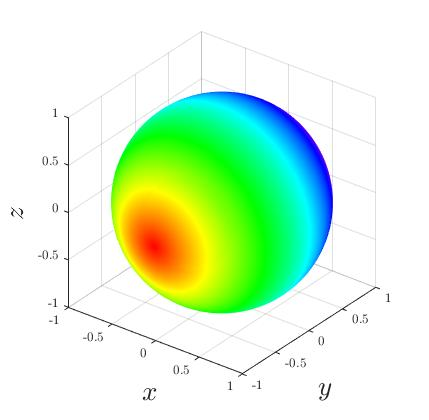
\includegraphics[width=\textwidth]{Figures/th}
		\caption{$\vartheta_i$ mapping}
		\label{subfig::theta_map}
	\end{subfigure}
	\begin{subfigure}{0.45\textwidth}
		\centering
		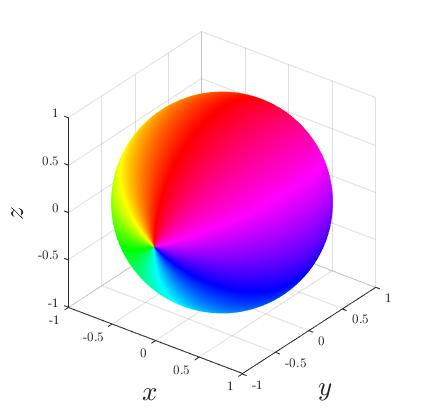
\includegraphics[width=\textwidth]{Figures/ph}
		\caption{$\varphi_i$ mapping}
		\label{subfig::phi_map}
	\end{subfigure}
	\caption{Possible values of $\vec q_i$ with color hue mapped to the values of $\vartheta_i$ in (\protect\subref{subfig::theta_map}) and $\varphi_i$ in (\protect\subref{subfig::phi_map})}
	\label{fig::singularities}
\end{figure}

\subsection{Reducing $w_i$}
We can also reduce each $\vec w_i$ to $\dot{\vartheta}_i$ and $\dot{\varphi}_i$.using the following equation which derives from equation \ref{eq::eom1} and the fact that $\vec q_i \cdot \vec w_i =0$:


\begin{equation}
	\vec w_i = \vec q_i \times \dot{\vec q}_i = 
	\begin{bmatrix} 
		\cos(\varphi_i)\\ 
		0\\ 
		\sin(\varphi_i) 
	\end{bmatrix}\dot\vartheta_i
	+
	\frac{1}{2}
	\begin{bmatrix} 
		\sin(2\,\vartheta_i)\,\sin(\varphi_i)\\ 
		-\cos(2\,\vartheta_i)-1\\ 
		-\sin(2\,\vartheta_i)\,\cos(\varphi_i) 
	\end{bmatrix}\dot\varphi_i
	\quad \foralli
	\label{eq::wi}
\end{equation}

These two reductions leave us with the following state vector:
\begin{equation}
	\vec{x}=
	[\vec p_l ,\quad
	\vartheta_1, \varphi_1, \vartheta_2, \varphi_2 \dots \vartheta_n,\varphi_n ,\quad
	\vec{\dot{p}}_l ,\quad
	\dot \vartheta_1,\dot \varphi_1, \dot \vartheta_2,\dot \varphi_2 \dots \dot \vartheta_n,\dot \varphi_n ,\quad
	\vec{ss}_1, \vec{ss}_2 \dots \vec{ss}_n
	]
	\label{eq::state}
\end{equation}

To use be able to generate the derivatives of the state vector (\ref{eq::state}) using the \ac{EOMs} we need to compute $\vec q_i$ and $\vec w_i$ using equations \ref{eq::qi} and \ref{eq::wi} respectively. We will also need to go from $\dot{\vec w}_i$ to $\ddot\vartheta$ and $\ddot\varphi$. 

In equation \ref{eq::qi} we can see that $\dot\vartheta_i$ is closely related to $\dot{\vec q}_i(2)$ and we can find that:
\begin{equation}
%	\dot{\vec q}_i(2)=\cos(\theta_i)\,\dot\theta_i
%	\rightarrow
%	\ddot{\vec q}_i(2)=\cos(\theta_i)\,\ddot \theta_i-\sin(\theta_i)\,{\dot \theta_i}^2
%	\rightarrow
	\ddot\vartheta_i=\frac{\sin(\vartheta_i)\,{\dot \vartheta_i}^2+\ddot{\vec q}_i(2)}{\cos(\vartheta_i)}
\quad\foralli
\end{equation}
Where $\ddot{\vec q}_i$ can be computed from $\dot{\vec w}_i$ using \ref{eq::eom1}:
\begin{equation}
	\ddot{\vec q}_i = \dot{\vec w}_i \times \vec q_i \, + \, \vec w_i \times \dot{\vec q}_i
\quad\foralli
\end{equation}
Similarly, in equation \ref{eq::wi} we can see that $\dot\varphi_i$ is closely related to $\vec w_i(2)$ and we can find that:
\begin{equation}
\ddot\varphi_i=\frac{\sin(2\,\vartheta_i)\,\dot \vartheta_i\,\dot \varphi_i-\dot{\vec w}_i(2)}{{\cos(\vartheta_i)}^2}
\quad\foralli
\end{equation}

\section{Slack Variables}
\label{sect::slack}
Slack variables are added to all inequalities in the MPC Problem. These variables have a very high cost added to them, this guarantees that they will always be zero if there are no problems. The purpose of these variables is to prevent the problem from having no solution and, therefore guaranteeing that the solver will always output something. For our problem we use: \lsymb{$s\in\R_{\ge0}$}{First slack variable} and \lsymb{$s_{env}\in\R$}{Second slack variable}. $s$ can only be positive, while $s_{env}$ can be any value, and they are used in different constraints (see section \ref{sect::constraints}). The vector concatenating both variables is denoted by \others{$\vec{s}\in\R^2$}{Slack variables}

\section{Forces PRO formulation}
Forces PRO uses the $\vec z$\hiddenlsymb{$\vec z\in\R^{3n+2+n_{var}}$}{asd} vector to represent stages. This vector is the concatenation of the $\vec{u}$, $\vec{s}$ and $\vec{x}$ vectors and has size $3n+2+n_{var}$.

\section{Constraints}
Constraints are very useful, we can use them to prevent the predicted system from behaving in ways that would be impossible for the real system. They also have low effect on the total time of the solver as, while they increase the time of each iteration, they also reduce the search space, reducing the number of iterations needed to find the optimal solution.

 
\label{sect::constraints}
\subsection{State Variables Restrictions}
\label{subsect::linear_ineq}
Some variables in the $\vec z$ vector are restricted by inequalities, in \cref{eq::linear_ineq} we can see all of these inequalities.

\begin{equation}
\begin{array}{r @{{}\le{}} c @{{}\le{}} l @{\qquad} l}
-15\degree & \bar \theta_i & 15\degree & \foralli\\
-15\degree & \bar \phi_i   & 15\degree & \foralli\\
\SI{-2}{\meter\per\second} & \bar{\dot z}_i & \SI{2}{\meter\per\second} & \foralli\\
0    & s        & \infty \\
-\infty & s_{env} & \infty \\
-60\degree & \vartheta_i & 60\degree & \foralli\\
-60\degree & \varphi_i   & 60\degree & \foralli\\
\end{array}
\label{eq::linear_ineq}
\end{equation}

%\subsection{Nonlinear inequalities}
%Nonlinear inequalities are applied to nonlinear functions. In Forces PRO these functions can depend on the $\vec z$ vector and a parameter vector that can be different on each stage. This vector will not be explained in detail, but is used to pass variables such as the predicted position of the obstacles, $\hat{\vec p}_{obs_i}$.

\subsection{Environment Constraints}
The drones and the payload must stay inside the environment. As the inequalities needed for this are bounded from both sides, we use $s_{env}$, as it can also be negative.

\begin{equation}
\begin{array}{r @{{}\le{}} c @{{}\le{}} l @{\qquad} l}

\begin{bmatrix}
-\frac{\vec{dim}(1)}{2}\\
-\frac{\vec{dim}(2)}{2}\\
0
\end{bmatrix}
&
\vec p_l + s_{env} 
&
\begin{bmatrix}
\frac{\vec{dim}(1)}{2}\\
\frac{\vec{dim}(2)}{2}\\
\vec{dim}(3)
\end{bmatrix} \\[30pt]
\begin{bmatrix}
-\frac{\vec{dim}(1)}{2}\\
-\frac{\vec{dim}(2)}{2}\\
0
\end{bmatrix}
&
\vec p_i + s_{env} 
&
\begin{bmatrix}
\frac{\vec{dim}(1)}{2}\\
\frac{\vec{dim}(2)}{2}\\
\vec{dim}(3) 
\end{bmatrix} & \foralli \\
\end{array}
\end{equation}

\subsection{Wire Slackening Prevention}
Our model does not take into account that the wire can be deformed or folded, instead, it is modeled as a solid beam. In early testing, it became apparent that the system was occasionally using the beams in order to push the payload, something impossible with wires. To prevent this from happening we need to add a constraint.

 According to the literature\cite{Pounds2012}, a wire goes from taunt to slack when the wire's tension becomes negative. Therefore we must prevent the wire from having a negative tension. To ensure this we find the force exerted by the \ac{EOMs} on each drone (denoted as \lsymb{$\vec T_i\in\R^3$}{Tension exerted on the $i$-th drone}) and add an extra inequality:
\begin{align}
 \vec T_i &= m_i\ddot{\vec p}_i - g\vec e_3 -\vec F_{uDi} \quad\foralli\\ 
0 &\le \vec q_i^T \vec T_i + s \quad\foralli	
\end{align}
\subsection{Drone Speed Limit}
We need to limit the drone speed to keep the movement safe. To do that we limit the drone speed:
\begin{equation}
\|\dot{\vec p}_i\|\le \SI{2}{\meter\per\second}\quad\foralli
\end{equation}
\subsection{Drone Distance}
We need to keep a minimum distance between drones so that they don't crash into each other:
\begin{equation}
\|\vec p_i - \vec p_j\|\ge \SI{0.4}{\meter}\quad\foralli\forallj
\end{equation}
\subsection{Collision Avoidance}
As explained in \cref{subsect::obstacle_modeling} (\nameref{subsect::obstacle_modeling}), the obstacles are modeled as a box. However, for collision avoidance, we will use the smallest volume ellipsoid that contains it. We do this because it is important for the equations of the \ac{MPC} to be as continuous as possible so that the solver converges on a solution faster.

Calculating distances from a point to an ellipsoid can be difficult, as seen in \cite{MAISONOBE2006}. However, we can use the approximation in equation 2-24 (given a point $[x,y,z]$ and an ellipsoid with center $[x_c,y_c,z_c]$ and sizes $a,b,c$). This approximation is good if you only want to check its sign.

\begin{equation}
d = 
\left(\frac{x-x_c}{a}\right)^2+
\left(\frac{y-y_c}{b}\right)^2+
\left(\frac{z-z_c}{c}\right)^2-1
\end{equation}

To calculate this approximated distance for the whole system, we find the distance between each of the wires and the expected position of the ellipsoid (assuming it follows linear movement) and find the minimum value. We also need to add some extra space to the ellipse to prevent a collision when the drones do not follow exactly the model.

To do this we need a way to calculate the distance between an ellipsoid and a segment. We use the same equation described in the Appendix C of \cite{Potdar2018}.

\section{Objective function}

The objective function consists of different objectives, each with their separate cost which are all added together using different weights. We will denote costs and their respective weights as \lsymb{$C_x$}{Cost of objective x} and \lsymb{$W_x$}{Weight of objective x}. Each cost is calculated for all stages of the prediction and added together, which is why a lot of the weights depend on the number of stages.

The objective function is really difficult to design, you can add a lot of different objectives to it and make the controller more complex and more intelligent. 

However, as you increase the complexity of the objective function is, the \ac{MPC} solver has more trouble finding its optimal value. It is also recommendable to keep the function as smooth as possible, preferably with a continuous derivative, as the \ac{MPC} solver relies on the derivatives to find the minimum.

This is why we will first introduce the most basic costs and more could be added if we had extra computational power.

\subsection{Destination Objective}

\begin{align}
C_{dest} & =
\sum_{i=0}^{n}\left(
(\vec p_i-\bar{\vec p}_i)^T
\begin{bmatrix}
1 & 0 & 0\\
0 & 1 & 0\\
0 & 0 & 1.1
\end{bmatrix}
(\vec p_i-\bar{\vec p}_i)\right)
\\
W_{dest} & = 
\begin{cases}
	5 & \text{if stage is final}
    \\ 0 & \text{otherwise}
\end{cases}
\end{align}

\subsubsection{Justification:}
The whole objective of the system is to go from one point to another. This is accomplished thanks to this objective.

Initially, we used the distance from the payload to the destination as an objective function, however, this poses a problem. The solver uses the inputs to minimize total cost, therefore it is best if the objective function is as closely related as possible to the inputs. This does not happen if we use the payload position, as the input force is applied to the drones, and then they pull from the payload.

Therefore we ended up using the distance between the drones and the desired position of the drones, which is computed from the desired position of the payload and desired suspension angles (using equations \ref{eq::pi} and \ref{eq::qi}).

In order to prevent discouraging the system from performing complex movements, such as moving away from the destination in order to dodge an obstacle, we will only optimize this objective for the final stage.

In order to get a simpler derivative of this cost term, we do not calculate the distance but the squared distance.

We also weight the $z$ coordinate of the distance slightly higher than the $x$ and $y$ coordinates so that the system tries to stay in the same horizontal plane as the objective if possible.

\subsection{Final Speed Minimization}
\begin{align}
C_{speed} & = \sum_{i=0}^{n}\left(
\vec{\dot p}_i^T
\vec{\dot p}_i
\right)
\\
W_{speed} & = 
\begin{cases}
10^{-2} & \text{if stage is final}
\\ 0 & \text{otherwise}
\end{cases}
\end{align}
\subsubsection{Justification:}
When the system can already reach the objective within the time-horizon, it is best to make sure that the final stage has also minimal velocity. This is not completely necessary, as we only use the first stages for drone input, however it makes the plan be more realistic. 

While using this cost across all stages would help stabilize the system, it is best not to do so as it is a really complex equation (we need to use \cref{eq::dqi} and the derivative of \cref{eq::pi}).

The weight is set very low to prevent this cost from discouraging movement.

It was also found that adding this cost increased convergence when the system is near the objective, as the last planner solution is more similar to the optimal plan.



\subsection{Input Minimization}
\begin{align}
C_{input} &=
\sum_{i=0}^{n}\left(
\vec u_i^T
\vec u_i \right)\\
W_{input} &=
\frac{10^{-2}}{N}
\end{align}

\subsubsection{Justification:}
The aim of this cost is to prevent the system from doing unnecessary movements, especially when it has already reached the destination. This helps stabilization and is really simple to calculate.

In order to prevent this cost from discouraging system movement, its weight is low compared to the other ones.


\subsection{Slack Minimization}
\begin{align}
C_{slack} &=
\vec{s}^T
\vec{s} \\
W_{slack} &=
\frac{10^{5}}{N}
\end{align}

\subsubsection{Justification:}
As explained in \cref{sect::slack} slack variables  should always be zero and this is accomplished by this cost. The weight of this should be really high, as slack variables only have to be used if it is impossible to find any other solution.
%%
% Setup
\chapter{System setup and control algorithm}

As explained in the introduction, the control of the algorithm is centralized, therefore a single agent controls the whole system. A \ac{MCS} is used to determine the position and attitude of the drones.

\label{chap::setup}
\section{Hardware and properties}
This is the hardware used in the thesis:
\setitemize{itemsep=-5pt}
\begin{itemize}
	\item \ac{MCS} by OptiTrack. The setup consists of 10 cameras filming at around \SI{120}{\hertz}.
	\item 4 Quadcopters (Bebop2 by Parrot, \Cref{fig::bebop}).
	\item 1 Gamepad (Logitech Wireless Gamepad F710, \Cref{fig::gamepad})
	\item Laptop (HP Pavilion 15-au007ns)
	\item Desktop computer (DELL OptiPlex 7050)
\end{itemize}

\begin{figure}
	\centering
	\begin{minipage}{.5\textwidth}
		\centering
		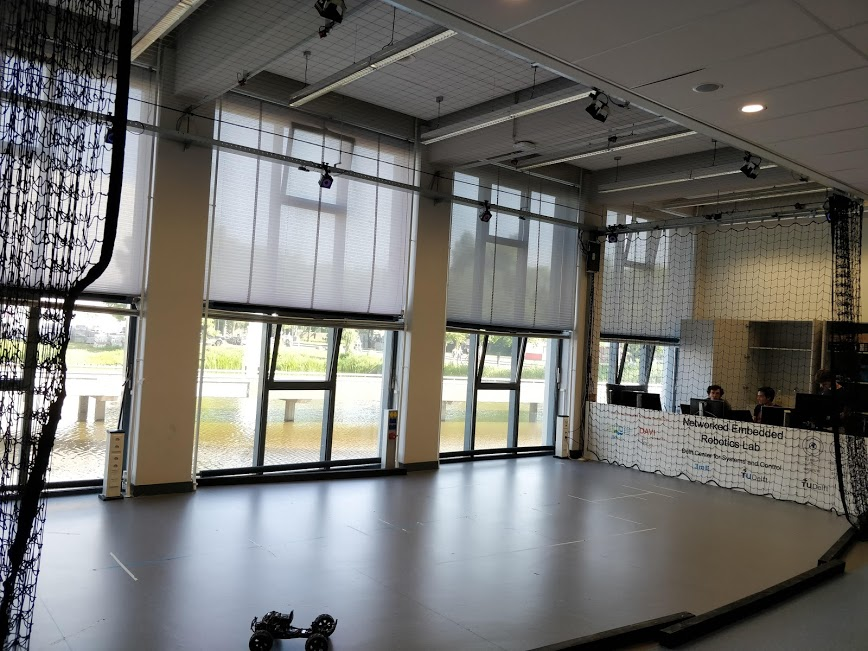
\includegraphics[width=1\linewidth]{Figures/workspace}
		\caption{Drones workspace}
		\label{fig::workspace}
	\end{minipage}%
	\begin{minipage}{.5\textwidth}
		\centering
		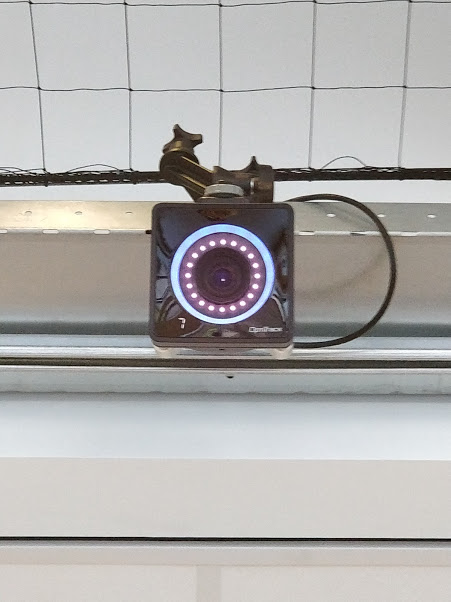
\includegraphics[width=.5\linewidth]{Figures/camera}
		\caption{\ac{MCS} camera}
		\label{fig::camera}
	\end{minipage}
\end{figure}

\begin{figure}
	\centering
	\begin{minipage}{.31\textwidth}
		\centering
		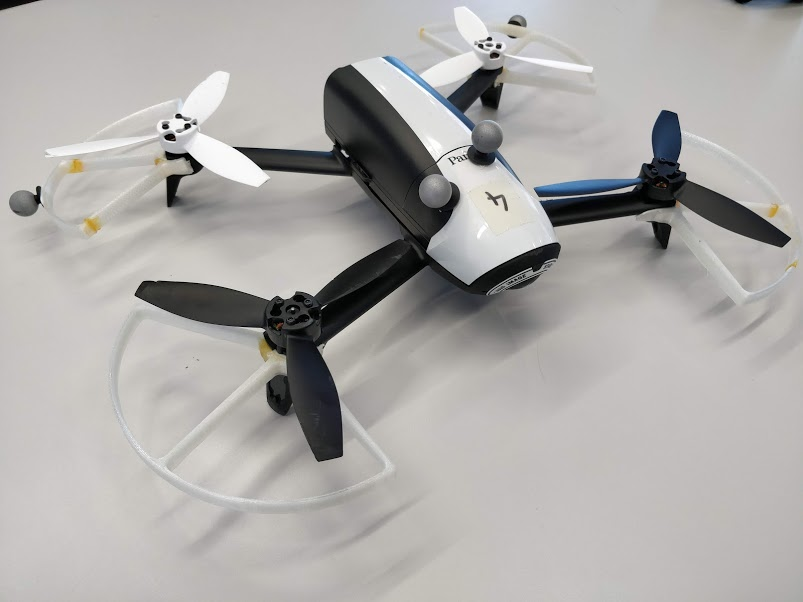
\includegraphics[width=.95\linewidth]{Figures/bebop}
		\caption{Bebop2 drone with markers}
		\label{fig::bebop}
	\end{minipage}%
	\begin{minipage}{.31\textwidth}
		\centering
		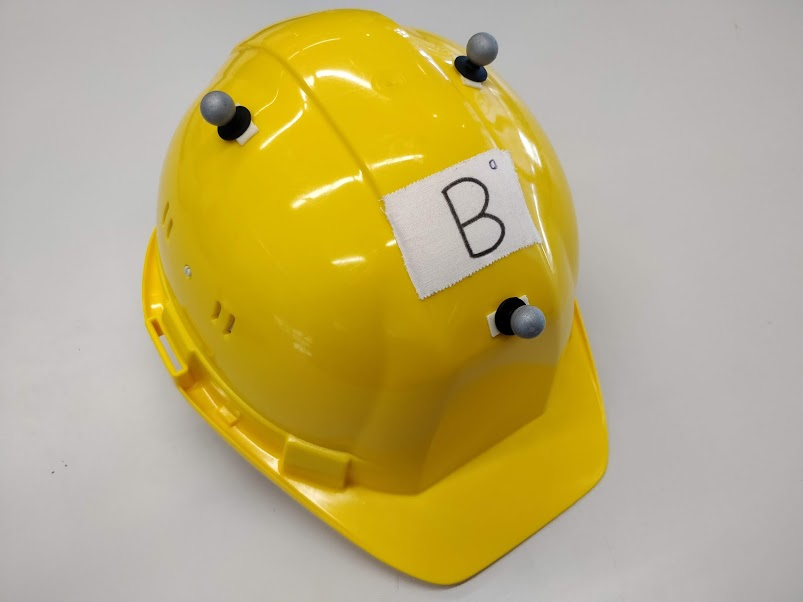
\includegraphics[width=.95\linewidth]{Figures/hat}
		\caption{Hat with reflective markers}
		\label{fig::hat}
	\end{minipage}%
	\begin{minipage}{.31\textwidth}
		\centering
		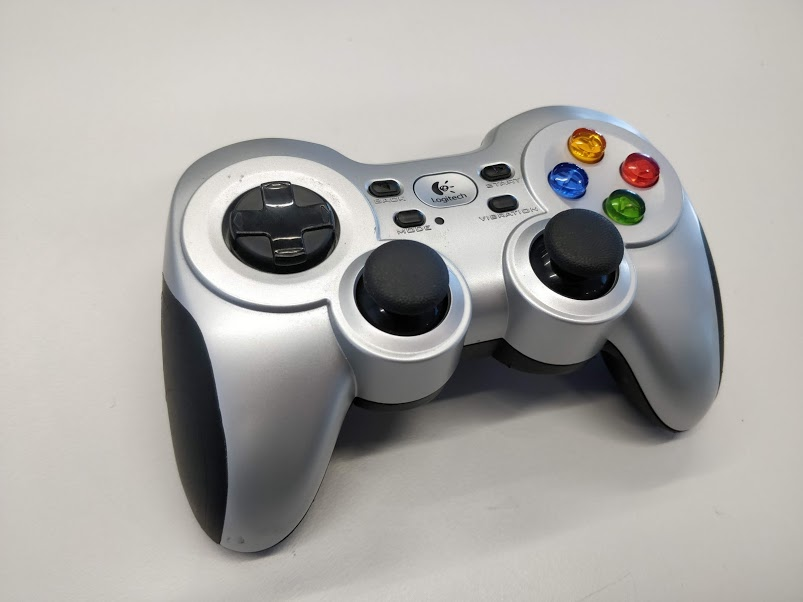
\includegraphics[width=.95\linewidth]{Figures/gamepad}
		\caption{Gamepad by Logitech}
		\label{fig::gamepad}
	\end{minipage}
\end{figure}

\section{Workspace}
The workspace of the drones, seen in  \cref{fig::workspace}, consists on a $6.0\times3.0\times2.6$ \si{\meter} $(L\times W\times H)$ arena where they can move freely while being tracked by the \ac{MCS}. The \ac{MCS} setup consists of 10 cameras such as the one seen in \cref{fig::camera}. The drones, payloads and obstacles are equipped with reflective markers to be tracked by the \ac{MCS}. The markers can be seen in figures \ref{fig::bebop} and \ref{fig::hat}.

\section{Control algorithm}
\label{sect::algorithm}
The basics of the control algorithm will be explained for simulation and the necessary extensions for the experimental setup will be explained in \cref{subsect::experimental_setup} (\nameref{subsect::experimental_setup}).

\subsection{Simulation Algorithm}
We use the following control algorithm: The system starts in a predefined position. Then, using FORCES PRO, a \ac{MPC} plan is generated such as the first stage equals the system state. 

The algorithm assumes that the system follows this plan for one time-step (of $\Delta t$) and calculates the new state using the \ac{EOMs}. The process is then repeated using the new state. A schematic of this solution can be seen in \cref{fig::initial_algorithm}.

During this process, obstacles are also simulated according to predefined movements (that the controller is not aware of).

This data is sent through \ac{ROS} to a visualizer, which will be further explained in \cref{sect::visualizer}


\subsubsection{External Planner}
An additional simulation algorithm was tested and, although it did not prove useful, we will also describe it.

The previous solution has a problem, if the \ac{MPC} solver takes a long time calculating the plan(longer than $1  / \Delta t$ \si{\second}) the simulation will run slower than real time and in the experimental setup the quadrotors will keep repeating the first input for longer than the planner intended. 

This can be solved if we separate the controller from the planner. The planner keeps re-planing using the controller's data as fast as possible, while the controller runs the simulation using inputs from the plan generated by the planner. 

To determine the inputs for each quadrotor, the controller finds the plan’s stage where the drone’s planned position is closest to the actual position. A schematic of this solution can be seen in \cref{fig::external_planner}.

When doing simulated experiments, it was found that cutting the maximum number of iterations of the \ac{MPC} solver in the initial algorithm was better than using an external planner.

\subsection{Initial Solution}
\label{subsect::initial_solution}
When solving the \ac{MPC} problem it is very important to give the solver a good initial solution. To do this we record the previous solution and update it for the next stage. 

If we are using the initial algorithm, the stage will be equal to the second stage in the previous \ac{MPC} solution. Therefore, we can shift the last solution by one stage and add a new stage at the end using the \ac{EOMs}.

\subsubsection{Initial Solution for the External Planner}
The above solution is not suitable for the external planner algorithm as the system could have gone through many stages of the plan.

To do this we compute the path that the controller would follow using the last solution using the same functions that the controller uses to determine the inputs from the plan. 

This initial solution is not good enough and is one of the main causes the external planner algorithm performs worse than the original algorithm.

\subsection{Experimental setup}
\label{subsect::experimental_setup}
As data from the drones tends to be inaccurate (it depends on GPS data and internal assumptions), we will use the \ac{MCS} to determine the position and attitude of the drones. 

A \ac{KF} is used to estimate the state of the system based on the \ac{EOMs} and the data from the \ac{MCS}. \ac{KF} is also used to estimate the location and velocity of the obstacles, which are also tracked with the \ac{MCS}.

\begin{figure}
	\centering
	\begin{minipage}{.5\textwidth}
		\centering
		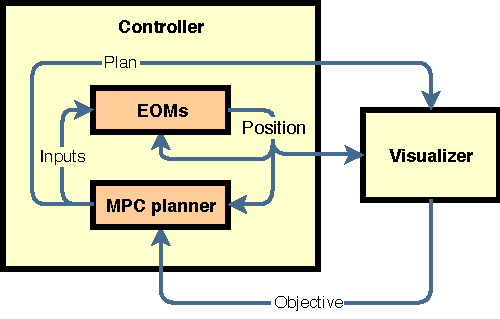
\includegraphics[width=.9\linewidth]{Figures/InitialAlgorithm}
		\caption{Simulation algorithm}
		\label{fig::initial_algorithm}
	\end{minipage}%
	\begin{minipage}{.5\textwidth}
		\centering
		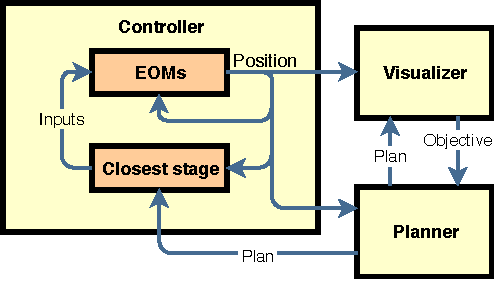
\includegraphics[width=.9\linewidth]{Figures/ExternalPlanner}
		\caption{External planner}
		\label{fig::external_planner}
	\end{minipage}
\end{figure}

\section{Data communication}
\label{sect::communication}
All data goes through the \ac{ROS} network, this means that we can separate different tasks throughout several computers and increase performance. The tasks are:
\begin{itemize}
	\item \textbf{\ac{ROS} core}: One of the computers has to start the \ac{ROS} core, this is a node that manages all communications through the \ac{ROS} network.
	\item \textbf{\ac{MCS} data}: Motive, a proprietary software by OptiTrack, computes the 3D location of the objects based on their markers. This data is then translated by a ROS node and fed to the ROS network.
	\item \textbf{Gamepad input}: A gamepad is connected to one computer through Bluetooth. A \ac{ROS} node in the same computer feeds the controller inputs to the \ac{ROS} network. The gamepad lets the user control the drones manually before turning on \ac{MPC}.
	\item \textbf{Drone commands}: Bebop2 drones create their own wireless network in order to communicate with other hardware. For each drone, a \ac{ROS} node receives commands from the \ac{ROS} network and sends them through the drone’s wireless network.
	\item \textbf{Controller}: As explained in more detail in \cref{sect::algorithm} (\nameref{sect::algorithm}), a controller written in \code{MATLAB} is in charge of getting the data from the \ac{MCS} and estimate the current state of the drones, payload and obstacles. Based on this information, it also generates the commands for the drone. If the experiment is running in simulation mode, this node is responsible for executing the simulation.
	\item \textbf{Planner}: As explained in more detail in \cref{sect::algorithm} (\nameref{sect::algorithm}), a planner written in \code{MATLAB} gets the position estimation from the controller and generates a plan for a fixed time horizon. Multiple planners can run at the same time.
	\item \textbf{Visualizer}: A visualizer, written in \code{MATLAB}, displays a \ac{GUI} with the estimated position of the system and the obstacles, as well as the latest plan. From the \ac{GUI} it is also possible to change the objective location which is shared through \ac{ROS}.
\end{itemize}
In \cref{fig::communications} a schematic for the whole control algorithm can be seen, including the communications for the experimental setup.



\begin{figure}
	\centering
	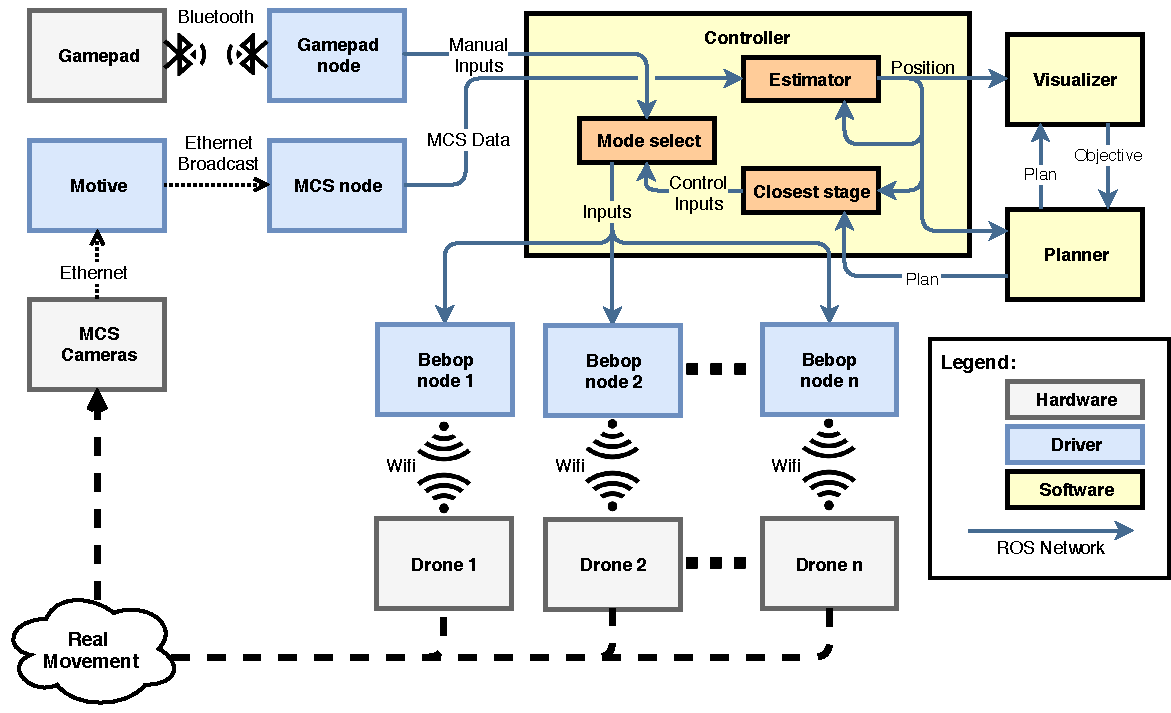
\includegraphics[width=1\linewidth]{Figures/Communications}
	\caption{Communications schematic}
	\label{fig::communications}
\end{figure}

\subsection{Rosbags}
One of the advantages of using \ac{ROS} for data communication is that we can use rosbags. Rosbags let us record all data into a file and then replay it. Even more, we can parse these files using \code{MATLAB} and analyze the data as we wish.

\section{Visualizer}
\label{sect::visualizer}
The visualizer is a \ac{GUI} created with \code{MATLAB}. A screenshot of the \ac{GUI} can be seen in \cref{fig::visualizer}. Through this interface we can:
\begin{itemize}
	\item See a representation of the system state and the obstacles in three dimensions.
		\subitem The drones are represented in black. 
		\subitem The wires are seen as blue lines.
		\subitem The payload is drawn as a red dot.
		\subitem The obstacles are displayed as gray boxes.
		\subitem The ellipsoids around the obstacle are shown as a brown surface.
		\subitem The planned trajectories of the drones are displayed as pink lines.
		\subitem The planned trajectory of the payload is shown as a dashed pink line.
		\subitem The current objective is drawn as a pink dot.
	\item See the numeric values of the current system state and inputs.
	\item Restart the simulated movement of the obstacles.
	\item Change the objective.
	\item Load and replay recorded data from a rosbag file.
\end{itemize}

\begin{figure}
	\centering
	\makebox[\textwidth][c]{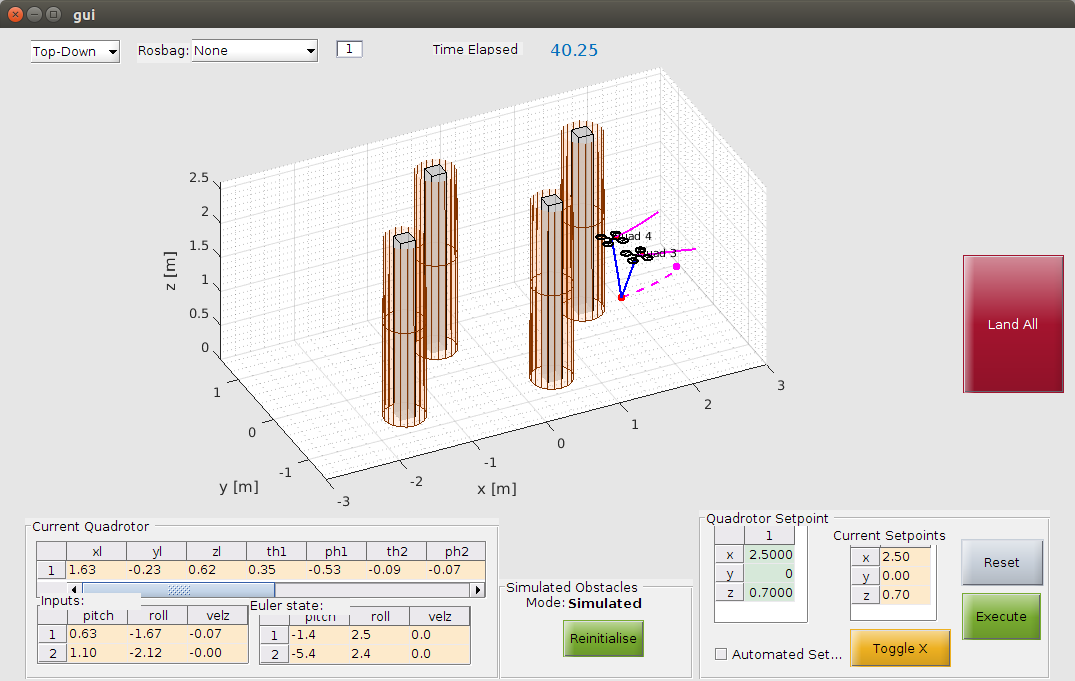
\includegraphics[width=1.2\linewidth]{Figures/visualizer}}
	\caption{Screenshot of the visualizer \ac{GUI}}
	\label{fig::visualizer}
\end{figure} 


%%
% Results
\chapter{Results} \label{chap::results}

\section{Simulation Scenario}
To do tests we use a simple scenario. Three static obstacles represent a fence which the system has to overcome. We set the simulation so that the drone has to move back and forth, jumping the fence several times, this is accomplished by switching the start and end points when the distance from the payload to the destination is less than \SI{.3}{\meter}. The simulation runs for \SI{20}{seconds} or until the solver cannot find a solution for 10 consecutive iterations. All the variables of the scenario can be seen in \cref{tab::scenario_data}. An example of a path taken by the system can be seen in \cref{fig::debug_log}.
\begin{table}
	\centering
	\resizebox{\columnwidth}{!}{
	\begin{tabular}{c | l*{14}{c}}
		Variable: & $n$ & $\vec{dim}$ & $\vec p_l$ &$\bar{\vec p}_l$ &  $\vartheta_1$ &  $\varphi_1$ & $\vartheta_2$ &  $\varphi_2$ & $\vec p_{obs_1}$ & $\vec{dim}_{obs_1}$ & $\vec p_{obs_2}$ & $\vec{dim}_{obs_2}$ & $\vec p_{obs_3}$ & $\vec{dim}_{obs_3}$ \\\hline
		\\[-10pt]
		Value: & $2$ & $\begin{bmatrix}
			6\\3\\2.6
		\end{bmatrix}$& $\begin{bmatrix}
		-2.5\\0\\.7
		\end{bmatrix}$& $\begin{bmatrix}
		2.5\\0\\.7
		\end{bmatrix}$
		& 45\degree & 0\degree & -45\degree & 0\degree & $\begin{bmatrix}
		0.01\\-1.2\\0.6
		\end{bmatrix}$ & $\begin{bmatrix}
		0.2\\ 0.2\\ 1.2
		\end{bmatrix}$ & $\begin{bmatrix}
		0.01\\1.2\\0.6
		\end{bmatrix}$ & $\begin{bmatrix}
		0.2\\ 0.2\\ 1.2
		\end{bmatrix}$  & $\begin{bmatrix}
		0.01\\.01\\0.5
		\end{bmatrix}$ & $\begin{bmatrix}
		1\\ 2.4\\ 1
		\end{bmatrix}$ 
		
	\end{tabular}
	}
	\caption{Simulation Scenario Data}
	\label{tab::scenario_data}
\end{table}

\begin{figure}
	\centering
	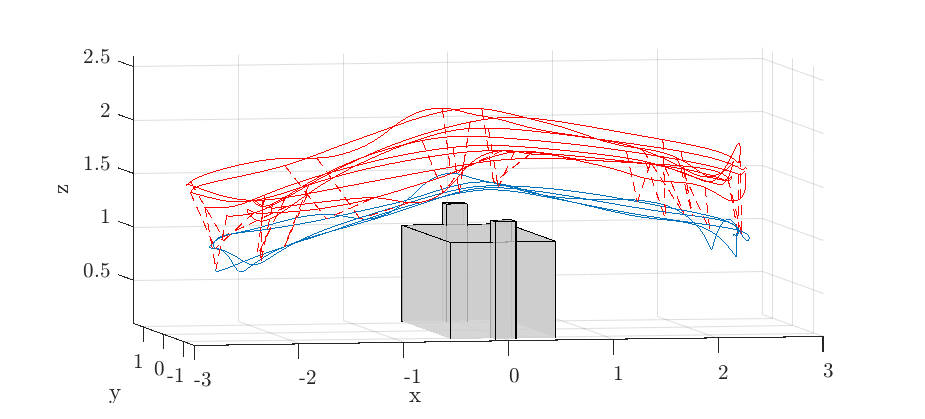
\includegraphics[width=.7\linewidth]{Figures/debug_log}
	\caption{Path of system with $N=20$, $\Delta t=.05$}
	\label{fig::debug_log}
\end{figure}

\section{Estimating time per iteration of the \ac{MPC} solver}
\label{subsect::time_per_it}
In order to set the maximum amount of iterations of the \ac{MPC} solver ($n_{maxit}$), we need to estimate the total time each iteration takes (denoted as \lsymb{$t_{it}$}{Time per iteration}). Even without access to the code from FORCES Pro, it is easy to guess that the time per iteration will depend linearly on the number of stages $N$ but it will not depend on $\Delta t$.

To check this assumption we run the experiments using the initial algorithm (no external planner) with $\Delta t\in\{.1,.05\}$ and $N\in\{10,11,14,17,20,24,29,34,41,50\}$ and on each step of each experiment we record the solve time and the number of iterations required by the solver. Then we plot the time per iteration divided by N using several box-plots. The results of this calculation can be seen in \cref{fig::time_per_it}.

\begin{figure}
	\centering
	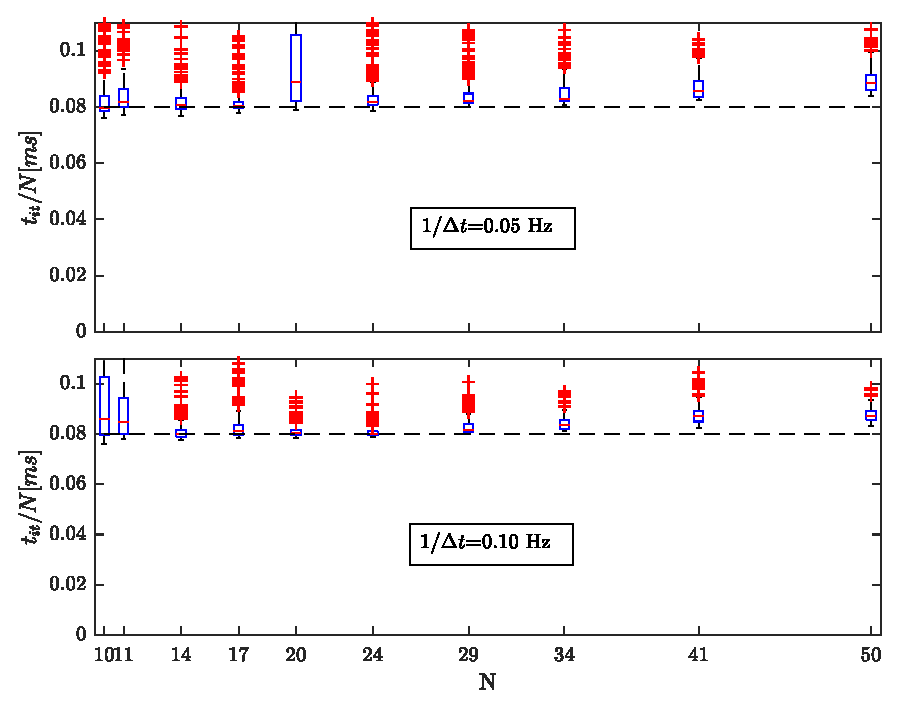
\includegraphics[width=.7\linewidth]{Figures/time_per_it}
	\caption[Graph of $t_{it}/N$]{\nameref{fig::time_per_it} \\ for $\Delta t\in\{.1,.05\}$ and $N\in\{10,11,14,17,20,24,29,34,41,50\}$ \\ A horizontal line is drawn at \SI{.08}{\milli\second}}
	\label{fig::time_per_it}
\end{figure}

Using these results we can see that most iterations run under \SI{.1}{\milli\second} per N, so we can set $n_{maxit}$ using the following equation:
\begin{equation}
\label{eq::maxit}
n_{maxit}=\left\lfloor\frac{\Delta t}{10^{-5}*N}\right\rfloor
\end{equation}

For a different number of drones or obstacles, it is clear that this constant will vary. However, we will not try to model this as the relation is non-linear. Ideally, it would be better to use a solver that can be limited by solve time instead of by the number of iterations. In \cref{fig::time_scaling_quad,fig::time_scaling_obs}, we can see how varying the number of drones or obstacles affects these times. 

\begin{figure}
	\centering
	\begin{minipage}{.5\textwidth}
		\centering
		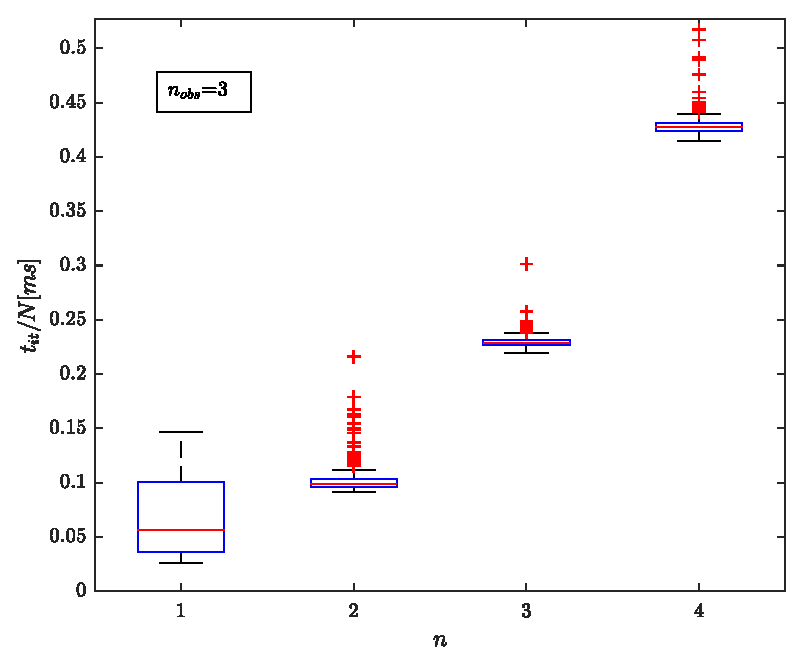
\includegraphics[width=.9\linewidth]{Figures/time_scaling_quad}
		\caption[Scaling of $t_{it}/N$ when varying $n$]{\nameref{fig::time_scaling_quad} with $n_{obs}=3$}
		\label{fig::time_scaling_quad}
	\end{minipage}%
	\begin{minipage}{.5\textwidth}
		\centering
		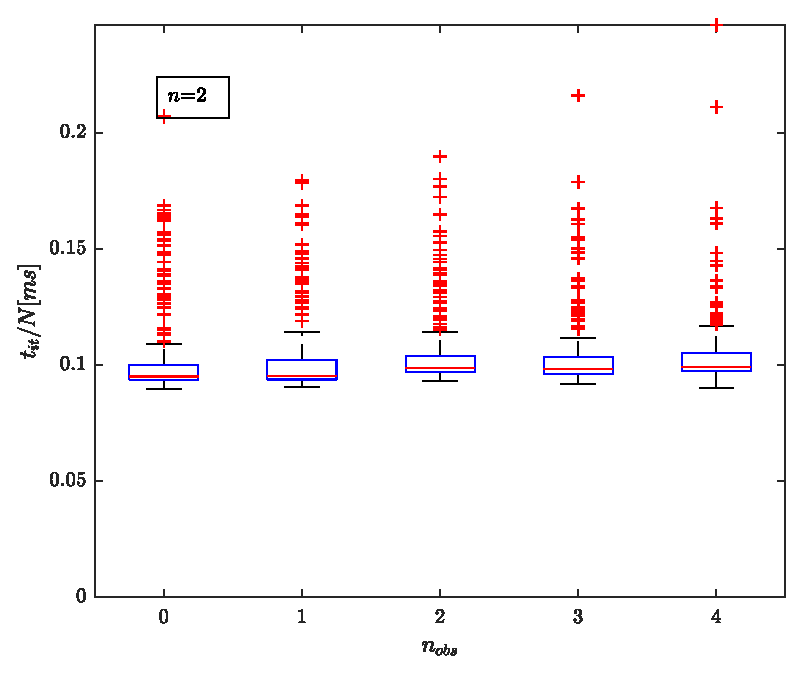
\includegraphics[width=.9\linewidth]{Figures/time_scaling_obs}
		\caption[Scaling of $t_{it}/N$ when varying $n_{obs}$]{\nameref{fig::time_scaling_obs} with $n=2$}
		\label{fig::time_scaling_obs}
	\end{minipage}
\end{figure}


\section{Step time outside the \ac{MPC} solver}
\label{sect::step_time}
When the $\Delta t$ is set to a low amount, the time of the functions other than the \ac{MPC} solver starts to be relevant. We can calculate this time subtracting the \ac{MPC} solve time (\lsymb{$t_{MPC}\in\R_+$}{MPC solve time}) from the time of the control loop (\lsymb{$t_{step}\in\R_+$}{Control loop time}) We calculated these times using the same parameters as the ones used in \cref{subsect::time_per_it}.

As it can be seen in \cref{fig::time_per_step}, these results do not seem to follow a pattern that is easy to model, so we will not try to model this and will assume that they are zero, this however will make the loop time slower than intended when setting $\Delta t$ to a small value.

\begin{figure}
	\centering
	\begin{center}
		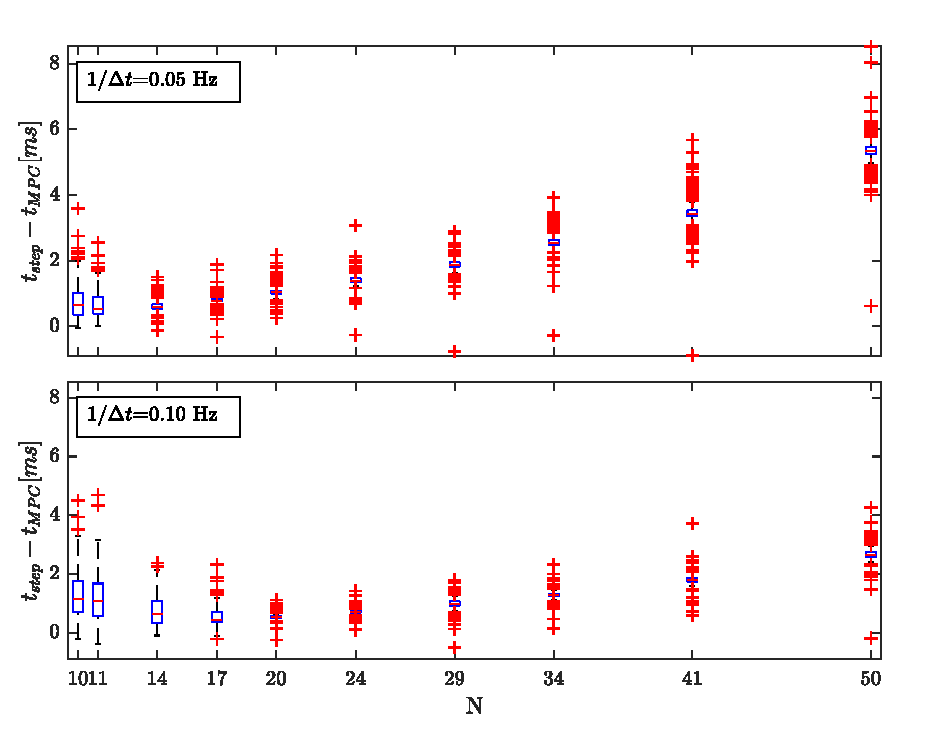
\includegraphics[width=.7\linewidth]{Figures/time_per_step}
	\caption[Graph of $t_{step}-t_{MPC}$]{\nameref{fig::time_per_step} \\ for $\Delta t\in\{.1,.05\}$ and $N\in\{10,11,14,17,20,24,29,34,41,50\}$}
	\label{fig::time_per_step}
	\end{center}
\end{figure}

\section{Finding best parameters}
We then ran some more tests to find the best parameters. We tested the same problem as in the previous sections with different $\Delta t$ and different time horizons (defined by $t_{horizon}=N\Delta t$ \hiddenlsymb{$t_{horizon}\in\R_+$}{Planning time horizon}). For each time horizon $N$ is found using the formula $N=\left\lceil\frac{t_{horizon}}{\Delta t}\right\rceil$. The results of these experiments are seen in \cref{fig::time_horizon}.

\Needspace{10\baselineskip}
From these results, and from further inspections on the data we concluded the following:
\begin{itemize}
	\item If the time horizon is too low, the system will break constraints more often. This makes sense as with a low time horizon the drone does not have time to react to the obstacles. As a good rule of thumb, the time horizon should be greater than the time needed for the system to stop.
	\item If the time horizon is too high the $N$ is high and following \cref{eq::maxit},$n_{maxit}$ will be smaller. Therefore, the quality of the results decrease (this cannot be seen in \cref{fig::time_horizon} but on inspection of the data obtained). 
	\item When the $\Delta_t$ is too high ($1/\Delta_t$ too low), the system tends to have more problems. This is mainly due to the errors that come from a rough discretization of the dynamics.
	\item When the $\Delta_t$ is too low ($1/\Delta_t$ too high), as explained on \cref{sect::step_time}, the loop time outside the \ac{MPC} solver will not be negligible and the loop will run slower than intended.
\end{itemize}

Taking into account all of this information, it was decided to have a time horizon of \SI{1.2}{\second} and a $\Delta t$ of \SI{0.083}{\second} (\SI{12}{\hertz}). Therefore the $N$ will have a value of $15$.

\begin{figure}
	\centering
	\begin{center}
		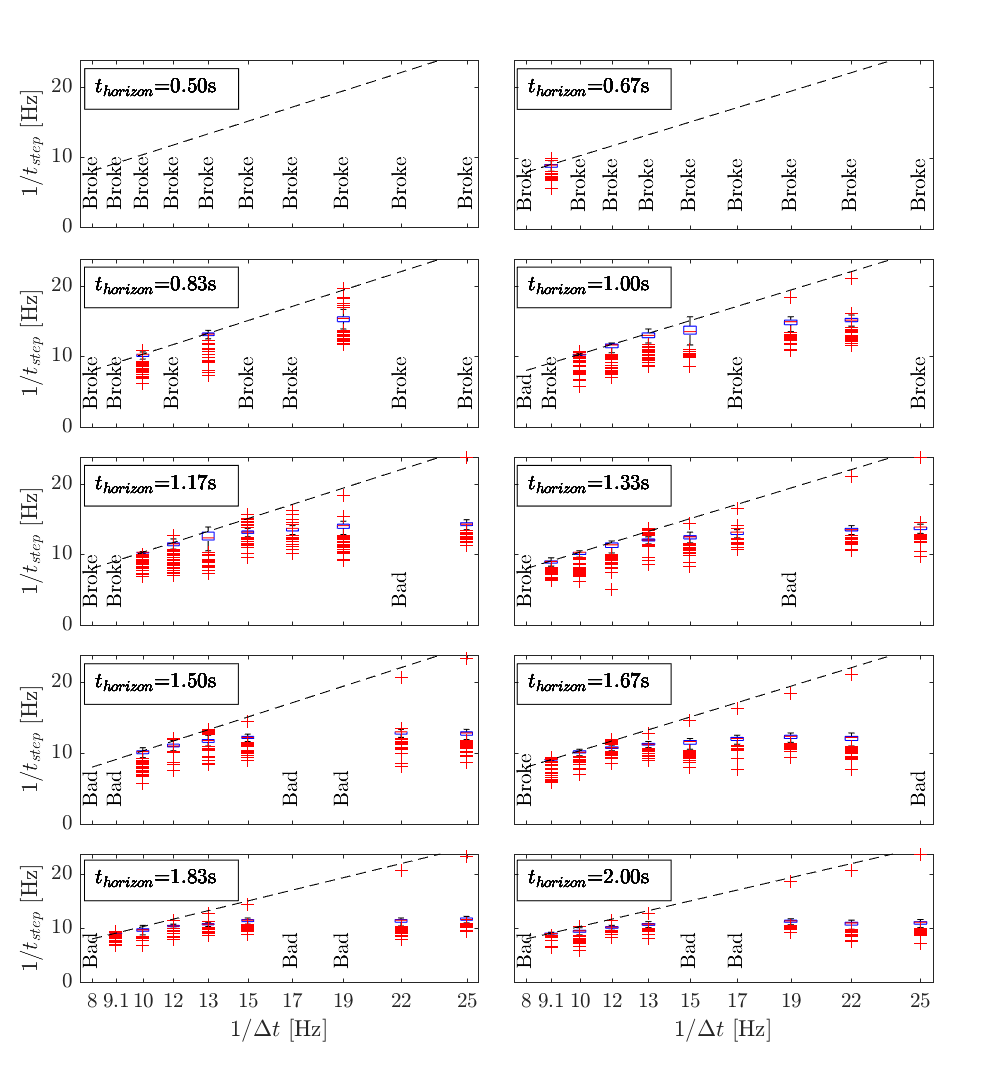
\includegraphics[width=1\linewidth]{Figures/time_horizon}
		\caption[Graph of $1/t_{step}$]{\nameref{fig::time_horizon} for $1/\Delta t\in\{8.0, 9.08, 10.3, 11.7, 13.3, 15.1, 17.1, 19.4, 22.0, 25.0\} \si{\hertz}$ and $t_{horizon}\in\{\frac{1}{2} , \frac{2}{3} , \frac{5}{6} , 1 , \frac{7}{6} , \frac{4}{3} , \frac{3}{2} , \frac{5}{3} , \frac{11}{6} , 2 \} \si{\second}$ \\ When the system broke any constraint for more than 1\% of the time it is marked as "Broke" \\When the system did not manage to cross the fence more than 3 times it is marked as "Bad" \\ A line marks the $t_{step}<\Delta t$ maximum.}
		\label{fig::time_horizon}
	\end{center}
\end{figure}

\section{External planner testing}
When we are using an external planner, we can no longer use the assumption that the drone has followed exactly the \ac{MPC} plan. Therefore we need to find the initial solution for the \ac{MPC} solver using the algorithm described in \cref{subsect::initial_solution}.

When testing the external planner algorithm we set the maximum number of iterations to a factor of the previous calculation. This factor, \lsymb{$k\in\R_+$}{Maximum iteration factor for external planner}, sets the maximum amount of stages the controller could perform without a new plan. 

\begin{equation}
\label{eq::maxit_k}
n_{maxit}=\left\lfloor\frac{k\Delta t}{10^{-5}*N}\right\rfloor
\end{equation}

As it was explained before, this algorithm was not successful, as it performed worse than the original algorithm. This was true for several values of k tested. The possible causes are:
\begin{itemize}
	\item The initial solution is poor, this means the solver takes more time to find the optimal solution and therefore, the next plan will have an even worse initial solution.
	\item The algorithm to determine the best inputs depending on the location of the drone does not perform well when the drone is far away from the plan.
	\item Even when the drone is in the path of the plan, it can be in between two of the planned stages, this causes the drone to follow inputs that were meant to be executed at a slightly different time.
\end{itemize}

\section{Demonstration of Maneuvers}
We will now demonstrate some maneuvers that our system is able to calculate. A video of these maneuvers can be seen in \url{https://youtu.be/lECcAQC_coE}.

\subsection{Moving obstacle avoidance}
To demonstrate moving obstacle avoidance a scenario is designed where two drones move from side to side while some obstacles move perpendicularly through the optimal path. 

In order to make it easier to visualize the movement from a top-down view, the obstacles are set to have a very large height, much larger than the workspace dimensions.

In \cref{fig::zigzag} we can see one of these maneuvers:

In (\ref{subfig::zigzag::start}) we see how the system is dodging obstacle 2. However, it is not doing anything to prevent a collision with obstacle 1, as it is not yet within the time horizon of the controller. 

In (\ref{subfig::zigzag::stop}) we see how obstacle 1 is now on the system's time horizon. Quadrotor 4 has already found a way to avoid the obstacle while quadrotor 3 is trapped, it cannot go forward as it assumes that the obstacle will be there in the future and it cannot turn to the right as it would crash against quadrotor 4, therefore the quadrotor 3 plans to stop as closely as possible to its objective. Also, note how quadrotor 3 stops in a way that makes the payload swing backward, avoiding a collision between the payload and the obstacle.

In (\ref{subfig::zigzag::found}) quadrotor 4 has followed its plan and is moving forward. This has given quadrotor 3 enough space to move behind quadrotor 4 and move towards its objective. Note how at the end of the planned path of quadrotor 3, it is not dodging the current position of the obstacle but its expected position.

Finally, in (\ref{subfig::zigzag::end}) we see how the system has successfully avoided the obstacle and is moving towards the objective.

\begin{figure}
	\centering
	\begin{subfigure}{0.45\textwidth}
		\centering
		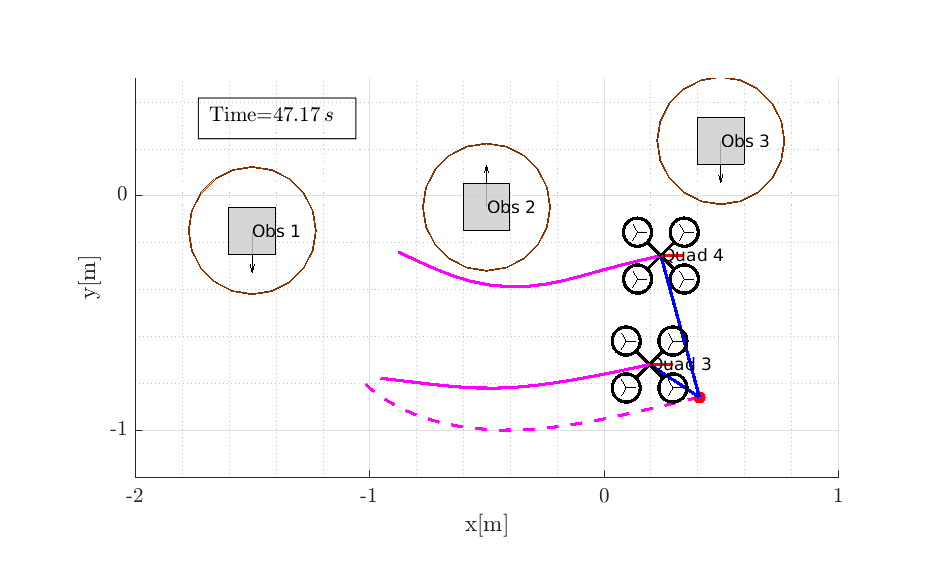
\includegraphics[width=\textwidth]{Figures/zigzag/start}
		\caption{Starting position of maneuver}
		\label{subfig::zigzag::start}
	\end{subfigure}
	\begin{subfigure}{0.45\textwidth}
		\centering
		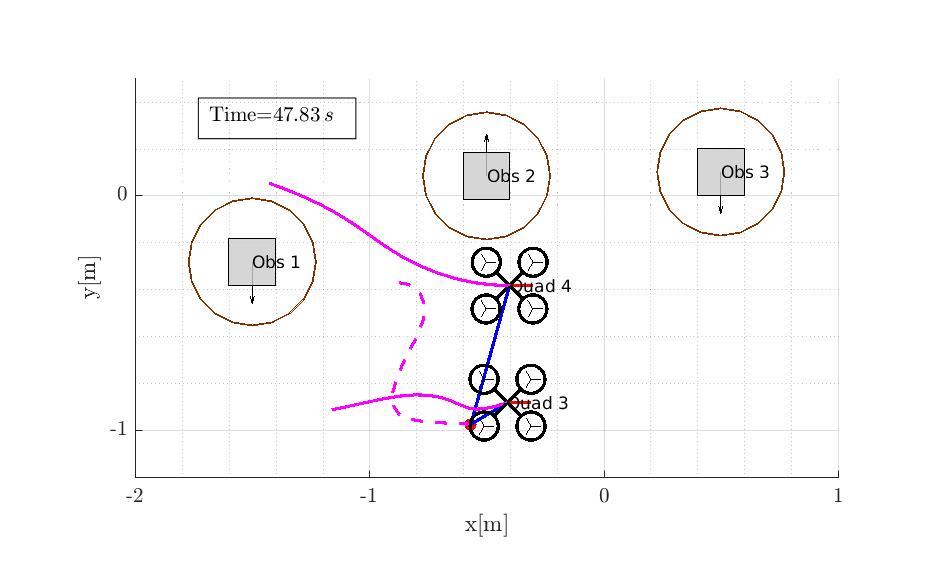
\includegraphics[width=\textwidth]{Figures/zigzag/stop}
		\caption{One drone stops}
		\label{subfig::zigzag::stop}
	\end{subfigure}
	\begin{subfigure}{0.45\textwidth}
		\centering
		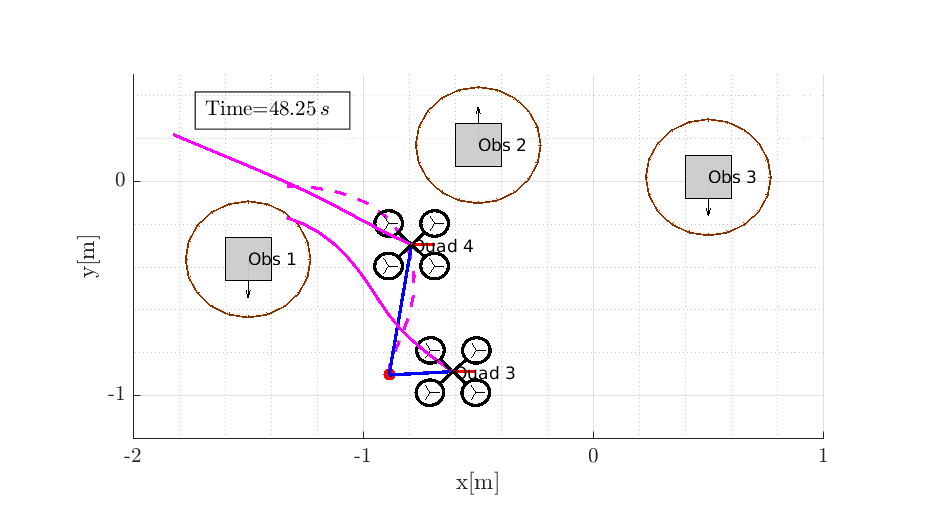
\includegraphics[width=\textwidth]{Figures/zigzag/found}
		\caption{A solution is found}
		\label{subfig::zigzag::found}
	\end{subfigure}
	\begin{subfigure}{0.45\textwidth}
		\centering
		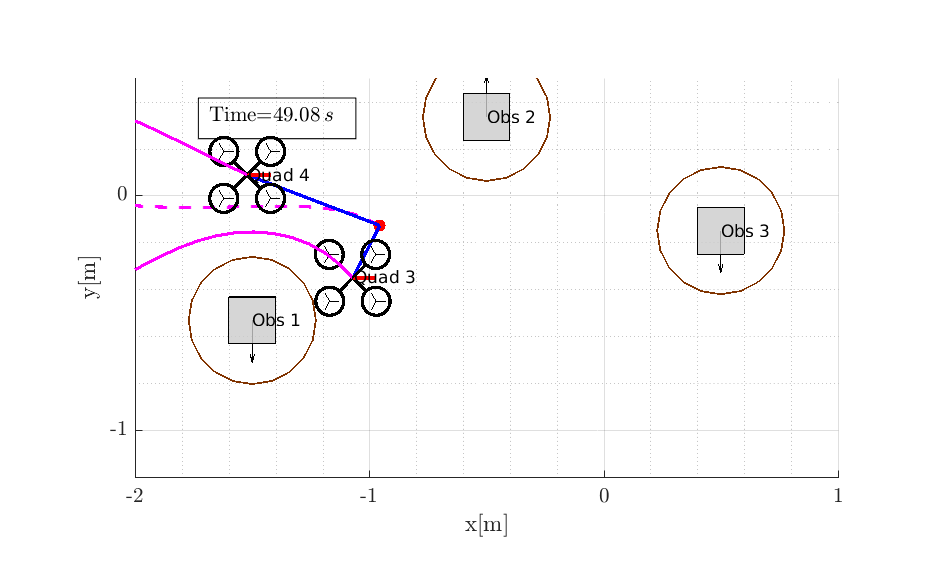
\includegraphics[width=\textwidth]{Figures/zigzag/end}
		\caption{The system avoids the obstacle}
		\label{subfig::zigzag::end}
	\end{subfigure}
	\caption[Moving obstacle avoidance]{\nameref{fig::zigzag}\\Plotted with the same rules as the ones explained in \cref{sect::visualizer} (\nameref{sect::visualizer})\\Black lines have been added to represent the obstacles' velocities\\For each instance, the top view is shown}
	\label{fig::zigzag}
\end{figure}

\subsection{High swing maneuvers}
In order to demonstrate maneuvers that utilize swing, we create a new scenario where two drones have to overcome a horizontal barrier that is in the way. To prevent the drones from simply going over it, we change the workspace limits to set a ceiling at a height of \SI{1}{\meter}. In order to exaggerate the movement, we increase the limit set to the swing angles in \cref{eq::linear_ineq} from \SI{60}{\degree} to \SI{85}{\degree}. 

In \cref{fig::highpole} we can see one of these maneuvers:


\begin{figure}
	\centering
	\begin{subfigure}{0.9\textwidth}
		\centering
		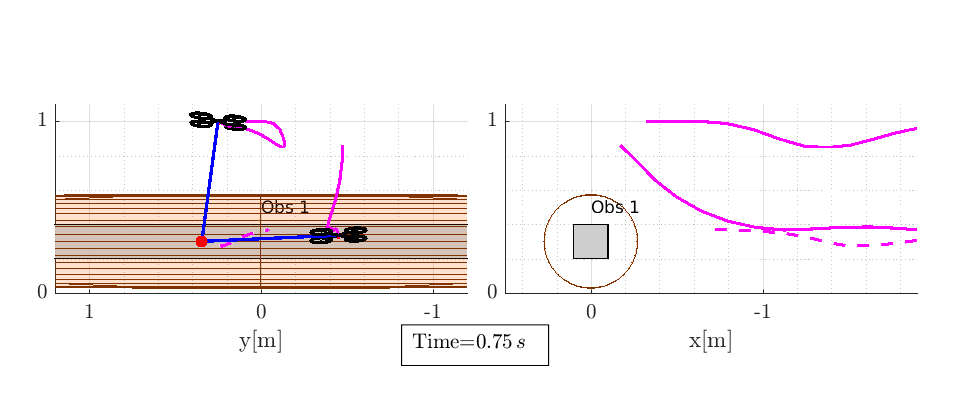
\includegraphics[width=\textwidth,trim={0 0 0 1cm},clip]{Figures/highpole/stop}
		\caption{The system does not yet know how to pass the obstacle}
		\label{subfig::highpole::stop}
	\end{subfigure}
	\begin{subfigure}{0.9\textwidth}
		\centering
		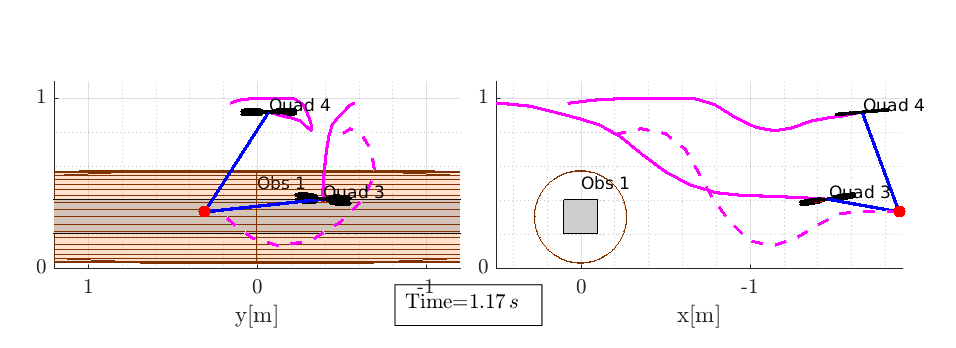
\includegraphics[width=\textwidth,trim={0 0 0 1cm},clip]{Figures/highpole/found}
		\caption{The system seems to have found a solution}
		\label{subfig::highpole::found}
	\end{subfigure}
	\begin{subfigure}{0.9\textwidth}
		\centering
		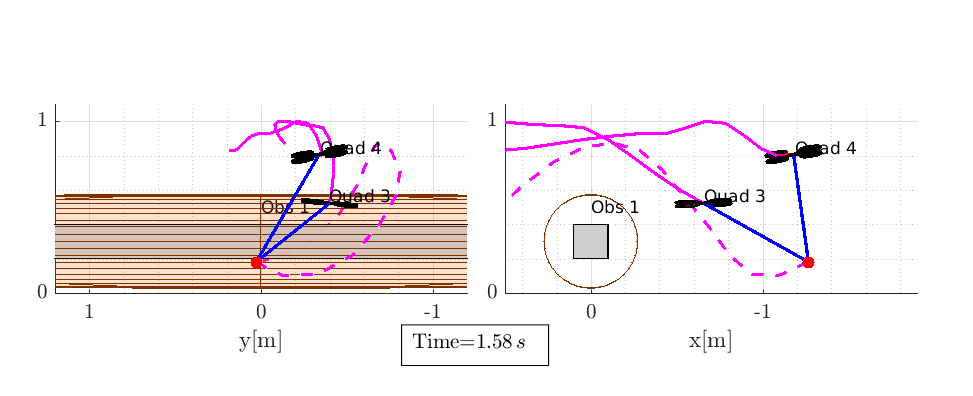
\includegraphics[width=\textwidth,trim={0 0 0 1cm},clip]{Figures/highpole/moving}
		\caption{The system moves closer}
		\label{subfig::highpole::moving}
	\end{subfigure}
	\begin{subfigure}{0.9\textwidth}
		\centering
		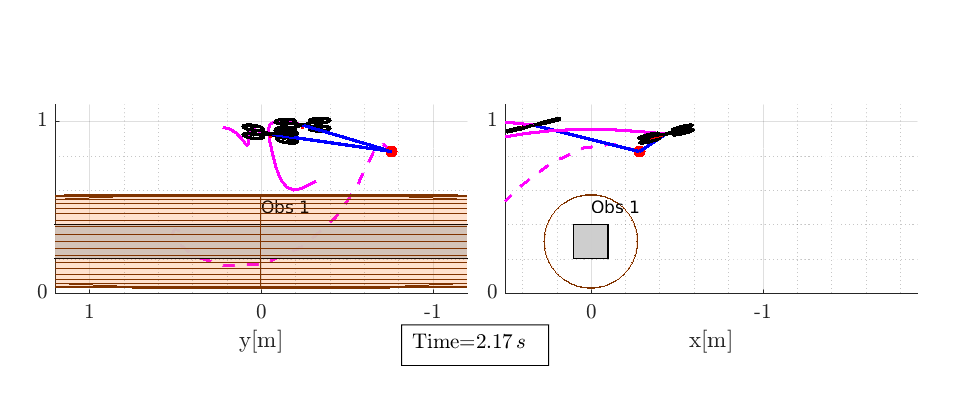
\includegraphics[width=\textwidth,trim={0 0 0 1cm},clip]{Figures/highpole/swing}
		\caption{The system swings the payload over the obstacle}
		\label{subfig::highpole::swing}
	\end{subfigure}
	\caption[High swing maneuver]{
		\nameref{fig::highpole}\\Plotted with the same rules as the ones explained in \cref{sect::visualizer} (\nameref{sect::visualizer}) \\ For each instance, two side views are shown}
	\label{fig::highpole}
	
\end{figure} 

In (\ref{subfig::highpole::stop}) the drones have just encountered the obstacle within the system's time horizon and have not yet found a solution to go over it, therefore the drones plan to get  as close as they can to the objective while staying behind the obstacle.

In (\ref{subfig::highpole::found}) the system seems to have found a solution to overcome the obstacle and the drones are starting to execute it.

In (\ref{subfig::highpole::moving}) the system has moved closer to the obstacle, and we can more clearly see what the plan was. Both drones have positioned themselves perpendicularly to the obstacle and are planning to swing the payload to the side while they go above the obstacle. This highly complex maneuver is only possible thanks to having a high time horizon and a good definition of the cost function.

In (\ref{subfig::highpole::swing}) we see how the payload is swinging above the obstacle and how each of the drone starts planning a path to move to their respective objectives.

\section{Experimental Results}
\label{sect::experimental}

Due to time limitations, very few experiments were performed with real drones and on none of them we got good enough results. 

Observing the logs of data obtained from these failures it was found that the system was generating correct \ac{MPC} plans and the system seemed to follow them correctly, which is promising. However, the length of the cables did not match the real distance between the payload and the quadrotors and, as in our model the position of the drones is determined by the position of the payload and the suspension angles (\cref{eq::pi}), this causes the position of the drones to be different in the model than in reality and the system destabilizes.

A boxplot of the real distances can be seen in \cref{fig::real_len}, we can see how these distances vary considerably. This is because the cables are not attached to the center of mass of the drones but to a different point. 

\begin{figure}
	\centering
	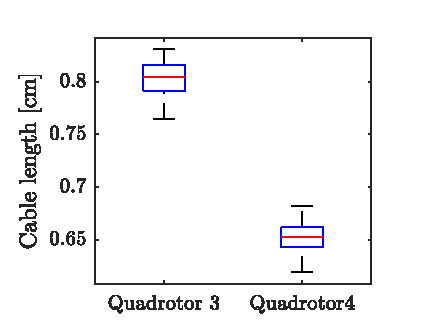
\includegraphics[width=.3\linewidth]{Figures/real_len}
	\caption{Real distance between the payload and the quadrotors} 
	\label{fig::real_len}
\end{figure}

With more time to experiment it could be possible to attach the drones differently or control the payload using longer cables so that this difference is minimized. Another solution would be to set the length of the cables as a parameter of the \ac{MPC} solver and set it to the real distance of the drones. It would also be a possibility to change the dynamic model to account for the difference the swing point of the cables and the center of mass of the quadrotors. A higher control rate would also help stabilize the system.


%%
% Conclusion
\chapter{Conclusion} \label{chap::conclusion}
In this thesis we introduced a new approach to the control of multiple \acp{UAV} carrying a slung payload through wires. This controller can be adapted to a variable number of quadrotors, obstacles and different environments. It is an agile controller able to generate complex maneuvers on the go even with uncertainties. It is able to dynamically adapt to changing environments, such as unexpected movement of obstacles or change of objective. The dynamic model is free of singularities, takes into account aerodynamic drag. Constraints prevent the system from doing unsafe movements and avoid wire slackening. The controller has been demonstrated to work in real-time simulated environments and the experiments on real drones, although unsuccessful, look promising.

\section{Future Studies}
For future studies we recommend the following:
\begin{itemize}
	\item Do more experimental studies of the controller.
	\item Test the system with a wider variety of parameters, such as heavier payloads or longer strings.
	\item For control of systems with more than three drones, it is almost impossible to prevent some of the wires from slackening, therefore a dynamic model that includes wire slackening would be preferred. Maybe a model where each of the wires can switch modes such as in \cite{Bisgaard2009}
	\item A more realistic model of the strings, where their mass is not neglected and they act more as springs rather than rigid cables would improve the accuracy of the dynamic equations.
	\item To improve realism and maybe fix the problems described in \cref{sect::experimental} it would be interesting to describe the string attachment points on the drone and on the payload.
	\item When the payload gets heavier, it would also be necessary to model it as a rigid body instead of as a point mass. This is done in \cite{Lee2014}.
	\item The complex dynamic equations could be substituted by some artificial intelligence which mimics the dynamic movement of the system.
	\item Drones with more direct inputs could be used so that we would not need to generate models of the internal dynamics.
	\item It would be ideal to switch the \ac{MPC} solver to one which can be limited by solve time instead of by the number of solver iterations.	
	\item An on-board control could be tested to rid the controller from the need of a \ac{MCS}.
	\item De-centralized control could be attempted for better scalability to an increase in the number of drones.
\end{itemize}

%
%
%========================== Appendices =======================================
\appendix

%\chapter{Project Planning}

\section{Planning and Scheduling}

The thesis started on \formatdate{1}{2}{2018} and will end on \formatdate{17}{6}{2018}, the week before the presentations start. This gives us an approximate project duration of 5 months.

The research is done in the laboratory at \ac{CoR} and an average of 40 hours a week are dedicated to the project.

Every two weeks, a meeting is scheduled with prof. Javier Alonso-Mora to demonstrate the work done and discuss the development of the project. The \ac{CoR} Department also has a monthly meeting where the projects of all students in \ac{CoR} are demonstrated and discussed.

This scheduling is not strictly enforced and will change depending on the availability of both the professor and me.

\section{Task Description}

\subsection{Paper reading}
Even before the project started, I began reading papers related to the thesis. Some were recommended by prof. Javier Alonso-Mora, such as the Master Thesis my project was going to be based on, by Nikhil D. Potdar \cite{Potdar2018}. I also read previous work by Alonso-Mora \cite{Alonso-Mora2017,Alonso-mora} and some related work such as Taeyoung Lee's work in \cite{Lee2013,Lee2014}

This reading had a duration of about two weeks and helped me better understand the work ahead of me and familiarize myself with how the problem could be solved.

\subsection{Installing and familiarizing myself with \ac{ROS}}
The next step was to install \ac{ROS} and understand how it worked. I chose to install \ac{ROS} Kinetic, as this was the version of \ac{ROS} used in the laboratory. This meant I had to do a fresh installation of \code{Ubuntu 16.04} as \ac{ROS} Kinetic only supports Wily (\code{Ubuntu 15.10}), Xenial (\code{Ubuntu 16.04}) and Jessie (\code{Debian 8}). To install \ac{ROS} I followed the instructions at \url{http://wiki.ros.org/kinetic/Installation/Ubuntu}.

To better understand \ac{ROS} I followed the official tutorials available at \url{http://wiki.ros.org/ROS/Tutorials}. I followed these tutorials until the intermediate level and tested my connection through the laboratory's Ethernet network.

I also Installed the ROS Drivers for the Drone which are available at \url{http://bebop-autonomy.readthedocs.io/en/latest/#} and the node for communication with the \ac{MCS}, which is available at \url{http://wiki.ros.org/mocap_optitrack}. I also tested communication with the drones and with the \ac{MCS}.

Finally, I installed \code{MATLAB} (version \code{R2017b}) and the \code{Robotics System Toolbox (version 1.4)} to communicate with \code{MATLAB} with the \ac{ROS} Network. I also did some tests to familiarize myself with the toolbox.

This process took about a week and a half, as I ran into problems with my \code{Ubuntu} installation and had to repeat the whole process several times.

\subsection{Understanding Nikhil D. Potdar's Code}
Nikhil D. Potdar's Thesis was in control of a single drone carrying a payload, and therefore, his code could be very useful for my research. This is why I dedicated some time to read through his code and understand every decision made in the code by reading his thesis \cite{Potdar2018} in a lot of detail. To get used to the code and better understand it I implemented some additional features on his code, such as inter-drone collision avoidance when multiple drones are carrying payloads. This process took two weeks.

\subsection{Finding an accurate dynamic model}
The next step was to find an accurate dynamic model for the multiple drone system. My first approach was to use something similar to what Nikhil D. Potdar used in his thesis, which consisted on defining the state using \code{MATLAB}'s symbolic toolbox and, calculating the Lagrangian $L$ of the system, and solving Lagrange's equation:
\begin{equation*}
\frac{d}{dt}
\left(
\frac{\partial L}{\partial \dot{\vec q}}
\right) - 
\frac{\partial L}{\partial \vec q}
= 0
\end{equation*}

However, as the multi-drone system was far more complex than the single-drone system, these equations were much more complex, this resulted in extremely long equations that were very badly optimized. I then tried to use Wolfram Mathematica's \code{FullSimplify} to simplify the equations, but they were so big that not even Mathematica could simplify them.

Finally, I used a different approach, I used the dynamic model introduced by Taeyoung Lee in \cite{Lee2013} and later simplified it for better performance. This task took approximately three weeks.

\subsection{Transforming Nikhil D. Potdar's Code for the multiple drone case}

The next step was to transform Nikhil D. Potdar's Code for the multiple drone case. The code had to be almost entirely rewritten, as a lot of parameters have to be added, the state vector and therefore, most of the functions have to be adapted to work with a variable amount of drones. The process is also very time consuming as the code uses a \ac{MPC} problem solver called FORCES PRO. This solver has to be generated every time a change is made in the \ac{MPC} problem and, as the equations are much more complex, FORCES PRO takes a really long time to generate a new solver.

The total time invested in this task was about two weeks.

\subsection{Adding constraints and tweaking cost function}
The \ac{MPC} problem has a lot of constraints and parameters that need to be tweaked and adjusted throughout the project. This task has been done in one week, but it continued throughout the project as new constraints came to my mind.

\subsection{Optimizing the code for real-time performance}
After transforming the code and running it in simulation, it became apparent that some optimization was required. Several methods  were applied, that will be explained further in the final thesis. This process is still ongoing at the time this report was written and its expected duration is of three weeks.

\subsection{Writing the thesis}
The thesis was written in parallel to many of the other tasks described previously, and will continue until the end of the project.

\subsection{Testing the planner in different scenarios}
When I am pleased with the results and speed of the planner, I will proceed to test it in different simulated scenarios. If I get a good enough planner speed in these scenarios, I will proceed to test it with real drones and document the results.

The expected duration of this process is of two weeks.

\section{Gantt chart}


\begin{figure}[H]
	\centering{}
	\def\gantttext{4cm}
	\begin{ganttchart}[
		time slot format=isodate,
		x unit = .85mm,
		y unit title = .7cm,
		y unit chart = .4cm,
		group label font = \tiny\bf,
		title label font = \tiny,
		bar label font = \tiny,
		vgrid={*{3}{draw=none},dotted,*{3}{draw=none}},
		today={\the\year-\the\month-\the\day},
		hgrid,
		calendar week text = {\currentweek},
		link bulge = 2,
		]{2018-02-1}{2018-06-29}
		\gantttitlecalendar{month=name, week} \\
		\node (a) [anchor=north east] at (current bounding box.north west){\tiny\textit{Month:}};
		\node (b) [anchor=south west] at (current bounding box.south west){\tiny\textit{Week:}};
		
		% Start gantt itself
		\ganttgroup{Preamble}{2018-02-01}{2018-03-11} \\
		\ganttbar{Paper reading}{2018-02-1}{2018-02-14} \\
		\ganttbar{ROS installation}{2018-02-15}{2018-02-25} \\
		\ganttlinkedbar{Understand code}{2018-02-26}{2018-03-11} \\
		
		
		\ganttgroup{Code development}{2018-03-12}{2018-05-13}\\
		\ganttlink{elem0}{elem4}
		\ganttbar{Dynamic model}{2018-03-12}{2018-04-1} \\
		\ganttlinkedbar{Transforming code}{2018-04-2}{2018-04-15} \\
		\ganttlinkedbar{Adding constraints}{2018-04-16}{2018-04-22} \\
		\ganttlinkedbar{Optimizing}{2018-04-23}{2018-05-13} \\
		
		\ganttgroup{Testing}{2018-05-28}{2018-05-41} \\
		\ganttlink{elem4}{elem9}
		\ganttbar{Testing}{2018-05-28}{2018-05-34} \\
		\ganttlinkedbar{Extract conclusions}{2018-05-35}{2018-05-41} \\
		
		\ganttgroup{Final Stage}{2018-04-16}{2018-06-29} \\
		\ganttbar{Write GEP report}{2018-05-14}{2018-05-27} \\
		\ganttbar{Write Thesis}{2018-04-16}{2018-05-13}
		\ganttbar{}{2018-05-28}{2018-06-17}\\
		\ganttbar{End project}{2018-06-18}{2018-06-24} \\
		\ganttbar{Presentation}{2018-06-25}{2018-06-29} \\
		
	\end{ganttchart}
	\caption{Gantt chart of the project \label{fig:gantt}}
\end{figure}
%


\chapter{Budget and Sustainability}


\section{Sustainability auto-evaluation}
When doing a project, there are several fields in which sustainability is necessary in order to prevent doing harm. Social sustainability is needed to maintain the lifestyle and health of our current society. Environmental sustainability helps keep our environment and, therefore, the planet in a good condition. Economic sustainability ensures the project will not be an economic failure.

In Information Technology projects, sustainability must also be considered, even if what you are creating is only software. Software can, for example, cause an increase in energy consumption (like Bitcoin) or not be profitable enough. That is why in this project it is also necessary to evaluate its impact on the planet. 

\section{Sustainability and Social Commitment}

\begin{table}[H]
\begin{center}
\begin{tabular}{|c|c|c|c|}
	\cline{2-4}
	\multicolumn{1}{c|}{} & \bf PPP & \bf Useful life & \bf Risks \\\hhline{-===}
	
	\multirow{2}{*}{\bf Environmental} & Design consumption & Ecological footprint & Environmental risks \\\cline{2-4}
	& 9/10 & 10/20 & -5/-20\\\hline
	
	\multirow{2}{*}{\bf Economical} & Bill & Viability plan & Economical risks \\\cline{2-4}
	& 5/10 & 15/20 & -3/-20\\\hline
	
	\multirow{2}{*}{\bf Social} & Personal impact & Social impact & Social risks \\\cline{2-4}
	& 7/10 & 19/20 & -4/-20\\\hline\hline
	
	\multirow{2}{*}{\bf Sustainability range} & 21/30 & 44/60 & -12/-60 \\\cline{2-4}
	& \multicolumn{3}{|c|}{53/90}\\\hline
	
\end{tabular}
\caption{Sustainability matrix of the project}
\label{tab::sustainability}
\end{center}
\end{table}

\subsection{Environmental Dimension}
During the research of the project, the amount of energy required is relatively low. We just need one computer, we can calculate it using my laptop's battery properties.
\begin{equation*}
\SI{19.5}{\volt} \cdot \SI{3.33}{\ampere} \cdot \SI{860}{\hour} = \SI{55.84}{\kilo\watt\hour}
\end{equation*}

We also need to charge the drones, which using the drone's battery properties we get:
\begin{equation*}
\SI[parse-numbers=true]{2700}{\milli\ampere\hour\per charge} \cdot \SI{11.1}{\volt} \cdot \SI{100}{charges} = \SI{3}{\kilo\watt\hour}
\end{equation*}

The rest of energy consumed, such as the \ac{MCS} and the laboratory lights are not included as they would be on even if the thesis would not have been developed. 

The total is \SI{58.84}{\kilo\watt\hour} which is extremely low compared to the amount consumed by the entirety humans in five months, which is \SI[parse-numbers=true]{71.2}{\peta\watt\hour}.

\subsection{Social Dimension}

As stated in the  \nameref{chap::intro} (chapter \ref{chap::intro}), the results from this thesis have a very big impact on social life, as it pushes forward a technology that would be very useful in many aspects of social life. The technology could be used to save lives in natural disasters and to make life easier in general.

As for the possible ethical implications, the only negative one is that the use of drones can also be used in military settings. However, this is something that is inevitable and researchers should not stop doing research because it might benefit the military.

\subsection{Economical Dimension}
In section \ref{sec::budget} (\nameref{sec::budget}) a detailed description of all the costs involved to make the research happen. In the long term, the project should have a positive impact in the economy, as it would mean smaller drones are required to do tasks that until now are done by bigger drones, reducing the cost of maintaining a fleet of drones.

\section{Project Budget}
\label{sec::budget}

\subsection{Hardware Budget}
To run the controller we need a laptop and the rest of the equipment is provided free of charge by the lab at \ac{CoR} and therefore does not affect the budget of the project.
Table \ref{budget::hardware} shows an estimation of the hardware costs related to the project. 

\begin{table}[H]
	\begin{center}
		\begin{tabular}{ |l|r|r|r|r| }
			\hline
			\bf Product & \bf Price & \bf Units  & \bf Useful Life & \bf Amortization \\\hline\hline
			HP Pavillion Laptop 15-au007ns & 800 \euro & 1  & 5 years & 67 \euro \\\hline  
			Laboratory equipment & 0 \euro & 1 & -- & -- \\\hline
			\bf Total:& 0 \euro & & & 67 \euro \\\hline
		\end{tabular}
		\caption{Hardware Budget}
		\label{budget::hardware}
	\end{center}
\end{table}

\subsection{Software Budget}
Table \ref{budget::software} shows the software used to develop this thesis. It is important to note that \code{Forces PRO} was used through a 6-months research license and \code{MATLAB} used a student license granted by \ac{FIB}.

\begin{table}[H]
	\begin{center}
		\begin{tabular}{ |l|r|r|r| }
			\hline
			\bf Product & \bf Price & \bf Units & \bf Amortization \\\hline\hline
			MATLAB and toolboxes & 0 \euro & 1 & 0 \euro \\\hline
			Forces PRO & 0 \euro & 1 & 0 \euro \\\hline
			\LaTeX & 0 \euro & 1 & 0 \euro \\\hline
			GitHub & 0 \euro & 1 & 0 \euro \\\hline
			GitKraken & 0 \euro & 1 & 0 \euro \\\hline
			\bf Total:& 0 \euro & & 0 \euro \\\hline
		\end{tabular}
		\caption{Software Budget}
		\label{budget::software}
	\end{center}
\end{table}

\subsection{Human Resources Budget}
In table \ref{task::time} we can find an estimation of the time required for each task. Using the totals of this estimation, we compute the Human Resources Budget in table \ref{budget::human}.

\begin{table}[H]
	\begin{center}
		\begin{tabular}{|l|r|r|r|r|}
			\hline
			\multirow{2}{*}{\bf Task} & \multirow{2}{*}{\bf Duration} & \multicolumn{3}{c|}{\bf Dedication}\\\cline{3-5}
			& & \bf Project Manager & \bf Software Developer & \bf Tester\\\hline\hline
			
			Paper reading & \SI{80}{\hour}& \SI{20}{\hour} & \SI{60}{\hour} & \\\hline
			
			ROS installation & \SI{60}{\hour}& \SI{15}{\hour} & \SI{45}{\hour} & \\\hline
			
			Understand code & \SI{80}{\hour}&  \SI{20}{\hour}&  \SI{60}{\hour}& \\\hline
			
			Dynamic model & \SI{120}{\hour}& \SI{30}{\hour} & \SI{60}{\hour} & \SI{30}{\hour} \\\hline
			
			Transforming code & \SI{80}{\hour}& \SI{20}{\hour} & \SI{40}{\hour} & \SI{20}{\hour} \\\hline
			
			Adding constraints & \SI{20}{\hour}& \SI{5}{\hour} & \SI{10}{\hour} & \SI{5}{\hour} \\\hline
			
			Optimizing & \SI{60}{\hour}& \SI{15}{\hour} & \SI{30}{\hour} & \SI{15}{\hour} \\\hline
			
			Testing & \SI{20}{\hour}& & & \SI{20}{\hour} \\\hline
			
			Extract conclusions & \SI{20}{\hour}& \SI{5}{\hour} & \SI{15}{\hour} & \\\hline
			
			Write GEP report & \SI{80}{\hour}& \SI{80}{\hour} & & \\\hline
			
			Write thesis & \SI{160}{\hour}& \SI{80}{\hour} & \SI{80}{\hour} & \\\hline
			
			End project & \SI{40}{\hour}& \SI{20}{\hour} & \SI{20}{\hour} & \\\hline
			
			Final Presentation & \SI{40}{\hour}& \SI{20}{\hour} & \SI{20}{\hour} & \\\hline\hline 
			
			\bf Total: & \SI{860}{\hour} & \SI{330}{\hour} & \SI{440}{\hour} & \SI{90}{\hour} \\\hline
		\end{tabular}
		\caption{Task Time Estimation}
		\label{task::time}
	\end{center}
\end{table}
\begin{table}[H]
	\begin{center}
		\begin{tabular}{ |l|r|r|r| }
			\hline
			\bf Role & \bf Hours & \bf \euro/hour & \bf Salary \\\hline\hline
			
			Project Manager & 330 & 35 & 11.550 \euro \\\hline
			
			Software Developer & 440 & 20 & 8.800 \euro \\\hline
			
			Tester & 90 & 15 & 1.350 \euro \\\hline\hline
			\bf Total: & 860 & --\, & 21.700 \euro \\\hline
		\end{tabular}
		\caption{Human Resources Budget}
		\label{budget::human}
	\end{center}
\end{table}


\subsection{Unexpected Costs}
In table \ref{budget::unexpected} we add any unexpected costs that might come up.

\begin{table}[H]
	\begin{center}
		\begin{tabular}{ |l|r|r|r| }
			\hline
			\bf Role & \bf Hours & \bf \euro/hour & \bf Salary \\\hline\hline
			
			Project Manager & 10 & 35 & 350 \euro \\\hline
			
			Software Developer & 20 & 20 & 400 \euro \\\hline
			
			Tester & 10 & 15 & 150 \euro \\\hline\hline
			
			\bf Total: & 860 & --\, & 900 \euro \\\hline
		\end{tabular}
		\caption{Unexpected Costs}
		\label{budget::unexpected}
	\end{center}
\end{table}

\subsection{Indirect Costs}

Other costs are included in table \ref{budget::indirect} but these were all provided by \ac{TU} and therefore do not affect the project's budget.

\begin{table}[H]
	\begin{center}
		\begin{tabular}{ |l|r|r|r| }
			\hline
			\bf Products & \bf Price & \bf Units & \bf Cost \\\hline\hline
			
			Electricity & \SI{0}{\EURO\per\kilo\watt\per\hour} & \SI{400}{\kilo\watt\hour} & 0 \euro \\\hline
			
			Internet & \SI{0}{\EURO\per month} & 5 months & 0 \euro
			
			\\\hline\hline
			\bf Total: & -- & --\, & 0 \euro \\\hline
		\end{tabular}
		\caption{Indirect Costs}
		\label{budget::indirect}
	\end{center}
\end{table}
\Needspace{20\baselineskip}
\subsection{Total Budget}
In table \ref{budget::total} we add all the budgets mentioned previously and a $5\%$ contingency for unexpected expenses.

\begin{table}[H]
	\begin{center}
		\begin{tabular}{|l|r|}
			\hline
			\bf Concept & \bf Estimated Costs\\\hline\hline
			
			Hardware & 67 \euro \\\hline
			Software & 0 \euro \\\hline
			Human Resources & 21.700 \euro \\\hline
			Unexpected Costs & 900 \euro \\\hline
			Indirect Costs & 0 \euro \\\hline
			\hline \bf Subtotal: & 22.600 \euro \\\hline
			
			Contingency ($5\%$)	& 1.130 \euro \\\hline
			\hline \bf Total: & \bf 23.730 \euro \\\hline
		\end{tabular}
		\caption{Indirect Costs}
		\label{budget::total}
	\end{center}
\end{table}



%\include{some chapter}

%========================== Back matter ======================================
\backmatter
%
% Bibliography
\bibliographystyle{ieeetr}
\bibliography{MyBib}
%
%
% Glossary
\chapter{Glossary} \label{chap::glossary}
%
\printacronyms
\begin{acronym}[\hspace{0.8in}] % 0.8in is also used by the nomenclature
	\acro{3mE}[3\textlarger{m}E]{Mechanical, Maritime and Materials Engineering}%
	\acro{AMS}{American Mathematical Society}%
	\acro{CoR}{Cognitive Robotics Department}%
	\acro{TU}[TU D\textlarger{elft}]{Delft University of Technology}%
	\acro{UPC}{Universitat Politècnica de Catalunya}
	\acro{FIB}{Facultat d'Informàtica de Barcelona}
	\acro{FME}{Facultat de Matemàtiques i Estadística}
	\acro{MAMME}{Master in Advanced Mathematics and Mathematical Engineering}
	\acro{IRI}{Institut de Robòtica i Informàtica Industrial}
	\acro{CFIS}{Centre de Formació Interdisciplinària Superior}
	\acro{AGAUR}{Agència de Gestió d'Ajuts Universitaris i de Recerca}
	\acro{UAV}{Unmanned Aerial Vehicle}
	\acro{MPC}{Model Predictive Control}
	\acro{NMPC}{Nonlinear Model Predictive Control}
	\acro{RK2}{2nd order Runge-Kutta}
	\acro{KF}{Kalman Filter}
	\acro{GUI}{Graphical User Interface}
	\acro{MCS}{Motion Capture System}
	\acro{ROS}{Robot Operating System}
	\acro{COM}{Center Of Mass}
	\acro{ENU}{East-North-Up}
	\acro{EOMs}{Equations of Motion}
	\acro{PID}{Proportional-Integral-Derivative}
\end{acronym}%
%
%
% Nomenclature
\newpage
\printnomencl%
%
% Index

\end{document}
